% ============================================================
%  Skrypt PrzeWrotka — Podstawy Kajakarstwa Górskiego
%  Plik główny — kompiluj ten plik w Overleaf
% ============================================================
\documentclass[12pt, a4paper]{article}

% --- Encoding & language ---
\usepackage[utf8]{inputenc}
\usepackage[T1]{fontenc}
\usepackage[polish]{babel}

% --- Layout ---
\usepackage[top=2.5cm, bottom=2.5cm, left=2.5cm, right=2.5cm]{geometry}
\usepackage{parskip}
\usepackage{microtype}

% --- Typography ---
\usepackage{lmodern}
\usepackage{titlesec}
\usepackage{enumitem}
\usepackage{booktabs}
\usepackage{tabularx}
\usepackage{longtable}
\usepackage{array}
\usepackage{multirow}

% --- Colours & boxes ---
\usepackage[dvipsnames]{xcolor}
\usepackage{tcolorbox}
\tcbuselibrary{skins}

% --- Figures ---
\usepackage{graphicx}
\usepackage{float}
\usepackage{caption}
\usepackage{chngcntr}
\usepackage{subcaption}
\counterwithin{figure}{section}   % figures numbered as 2.1, 2.2, 3.1 …

% --- Hyperlinks ---
\usepackage[hidelinks]{hyperref}

% ============================================================
%  Colours
% ============================================================
\definecolor{clubblue}{HTML}{1A5276}
\definecolor{clubgray}{HTML}{F2F3F4}
\definecolor{tiphint}{HTML}{D6EAF8}
\definecolor{warnred}{HTML}{FDEDEC}
\definecolor{warnframe}{HTML}{C0392B}

% ============================================================
%  Section formatting
% ============================================================
\titleformat{\section}
  {\Large\bfseries\color{clubblue}}
  {\thesection.}{0.8em}{}[\titlerule]

\titleformat{\subsection}
  {\large\bfseries\color{clubblue!80!black}}
  {\thesubsection.}{0.6em}{}

\titleformat{\subsubsection}
  {\normalsize\bfseries}
  {\thesubsubsection.}{0.5em}{}

% ============================================================
%  Blank figure placeholder
%  Usage: \placeholder{width}{height}{caption}
% ============================================================
\newcommand{\placeholder}[3]{%
  \begin{figure}[H]
    \centering
    \fcolorbox{clubblue!50}{clubgray}{%
      \parbox[c][#2][c]{#1}{%
        \centering\color{clubblue!70}\small[Miejsce na zdjęcie / rysunek]%
      }%
    }
    \caption{#3}
  \end{figure}%
}

% ============================================================
%  Tip box  —  tip.png must be uploaded to Overleaf project
% ============================================================
\newtcolorbox{tipbox}{
  colback=tiphint, colframe=clubblue!60,
  fonttitle=\bfseries,
  title={
\includegraphics[height=1em]{tip.png}\enspace Wskazówka},
  left=4pt, right=4pt, top=4pt, bottom=4pt
}

% ============================================================
%  Warning box
% ============================================================
\newtcolorbox{warnbox}{
  colback=warnred, colframe=warnframe,
  fonttitle=\bfseries\color{warnframe}, title=Uwaga,
  left=4pt, right=4pt, top=4pt, bottom=4pt
}

% ============================================================
\begin{document}
% ============================================================

% ---- Title page ----
\begin{titlepage}
  \centering
  \vspace*{\fill}
  
\includegraphics[width=\linewidth]{images/front_cover.png}
  \vspace*{\fill}
\end{titlepage}

\newpage
\tableofcontents
\newpage

% ---- Chapters ----
% ============================================================
%  Rozdział 1 — Wstęp
% ============================================================
\section{Wstęp}

Cześć! Bardzo miło Cię poznać i cieszymy się całym klubem, że zdecydowałeś/aś się na wzięcie udziału w szkoleniu.

Pamiętaj, że to dopiero początek Twojej przygody i ogrom wiedzy do zdobycia. Ponieważ jest to kurs podstawowy, w skrypcie znajdziesz podstawowe informacje — jak w szkole podstawowej. Uczymy się całe życie, więc cała edukacja teoretyczna i przede wszystkim praktyczna jest przed Tobą. Trzymam za Ciebie kciuki i na pewno nie pożałujesz decyzji o wzięciu udziału w kursie!
% ============================================================
%  Rozdział 2 — Sprzęt
% ============================================================
\section{Sprzęt}

% ------------------------------------------------------------
\subsection{Kajak i pozycja w kajaku}
% ------------------------------------------------------------

Nazwy części kajaka, których warto się nauczyć (bo często się powtarzają):

\begin{itemize}[leftmargin=1.5em, itemsep=2pt]
  \item \textbf{dziób} — przód
  \item \textbf{rufa} — tył
  \item \textbf{kokpit} — otwór wejściowy
  \item \textbf{podnóżek} — oparcie na stopy
  \item \textbf{boczki} — przylegają do bioder
  \item \textbf{motylki} — przylegają do wewnętrznej strony kolan
  \item \textbf{oparcie}
\end{itemize}

\begin{figure}[h]
    \centering
    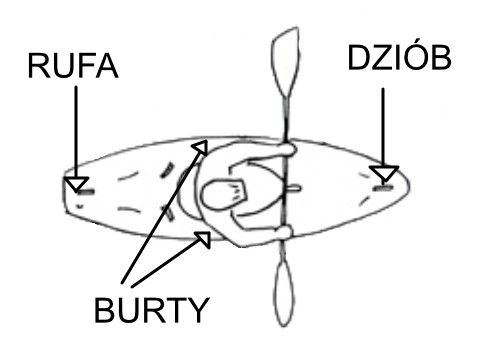
\includegraphics[width=200px]{images/schemat_budowy_kajaka.jpg}
    \caption{Schemat budowy kajaka z opisanymi częściami}
\end{figure}

\textbf{Pozycja.}
Kajakarz siedzi na „żabę" — stopy powinny całą powierzchnią opierać się o podnóżek.Podnóżek musi być solidny, najczęściej wykonany z płyty aluminiowej bądź tworzywa, czasami z pianki wypełniającej cały dziób. Należy zwrócić uwagę, że bardzo niebezpieczne jest wpadnięcie stopy za podnóżek - musi być on tak dopasowany, aby było to absolutnie niemożliwe.

\begin{figure}[h]
    \centering
    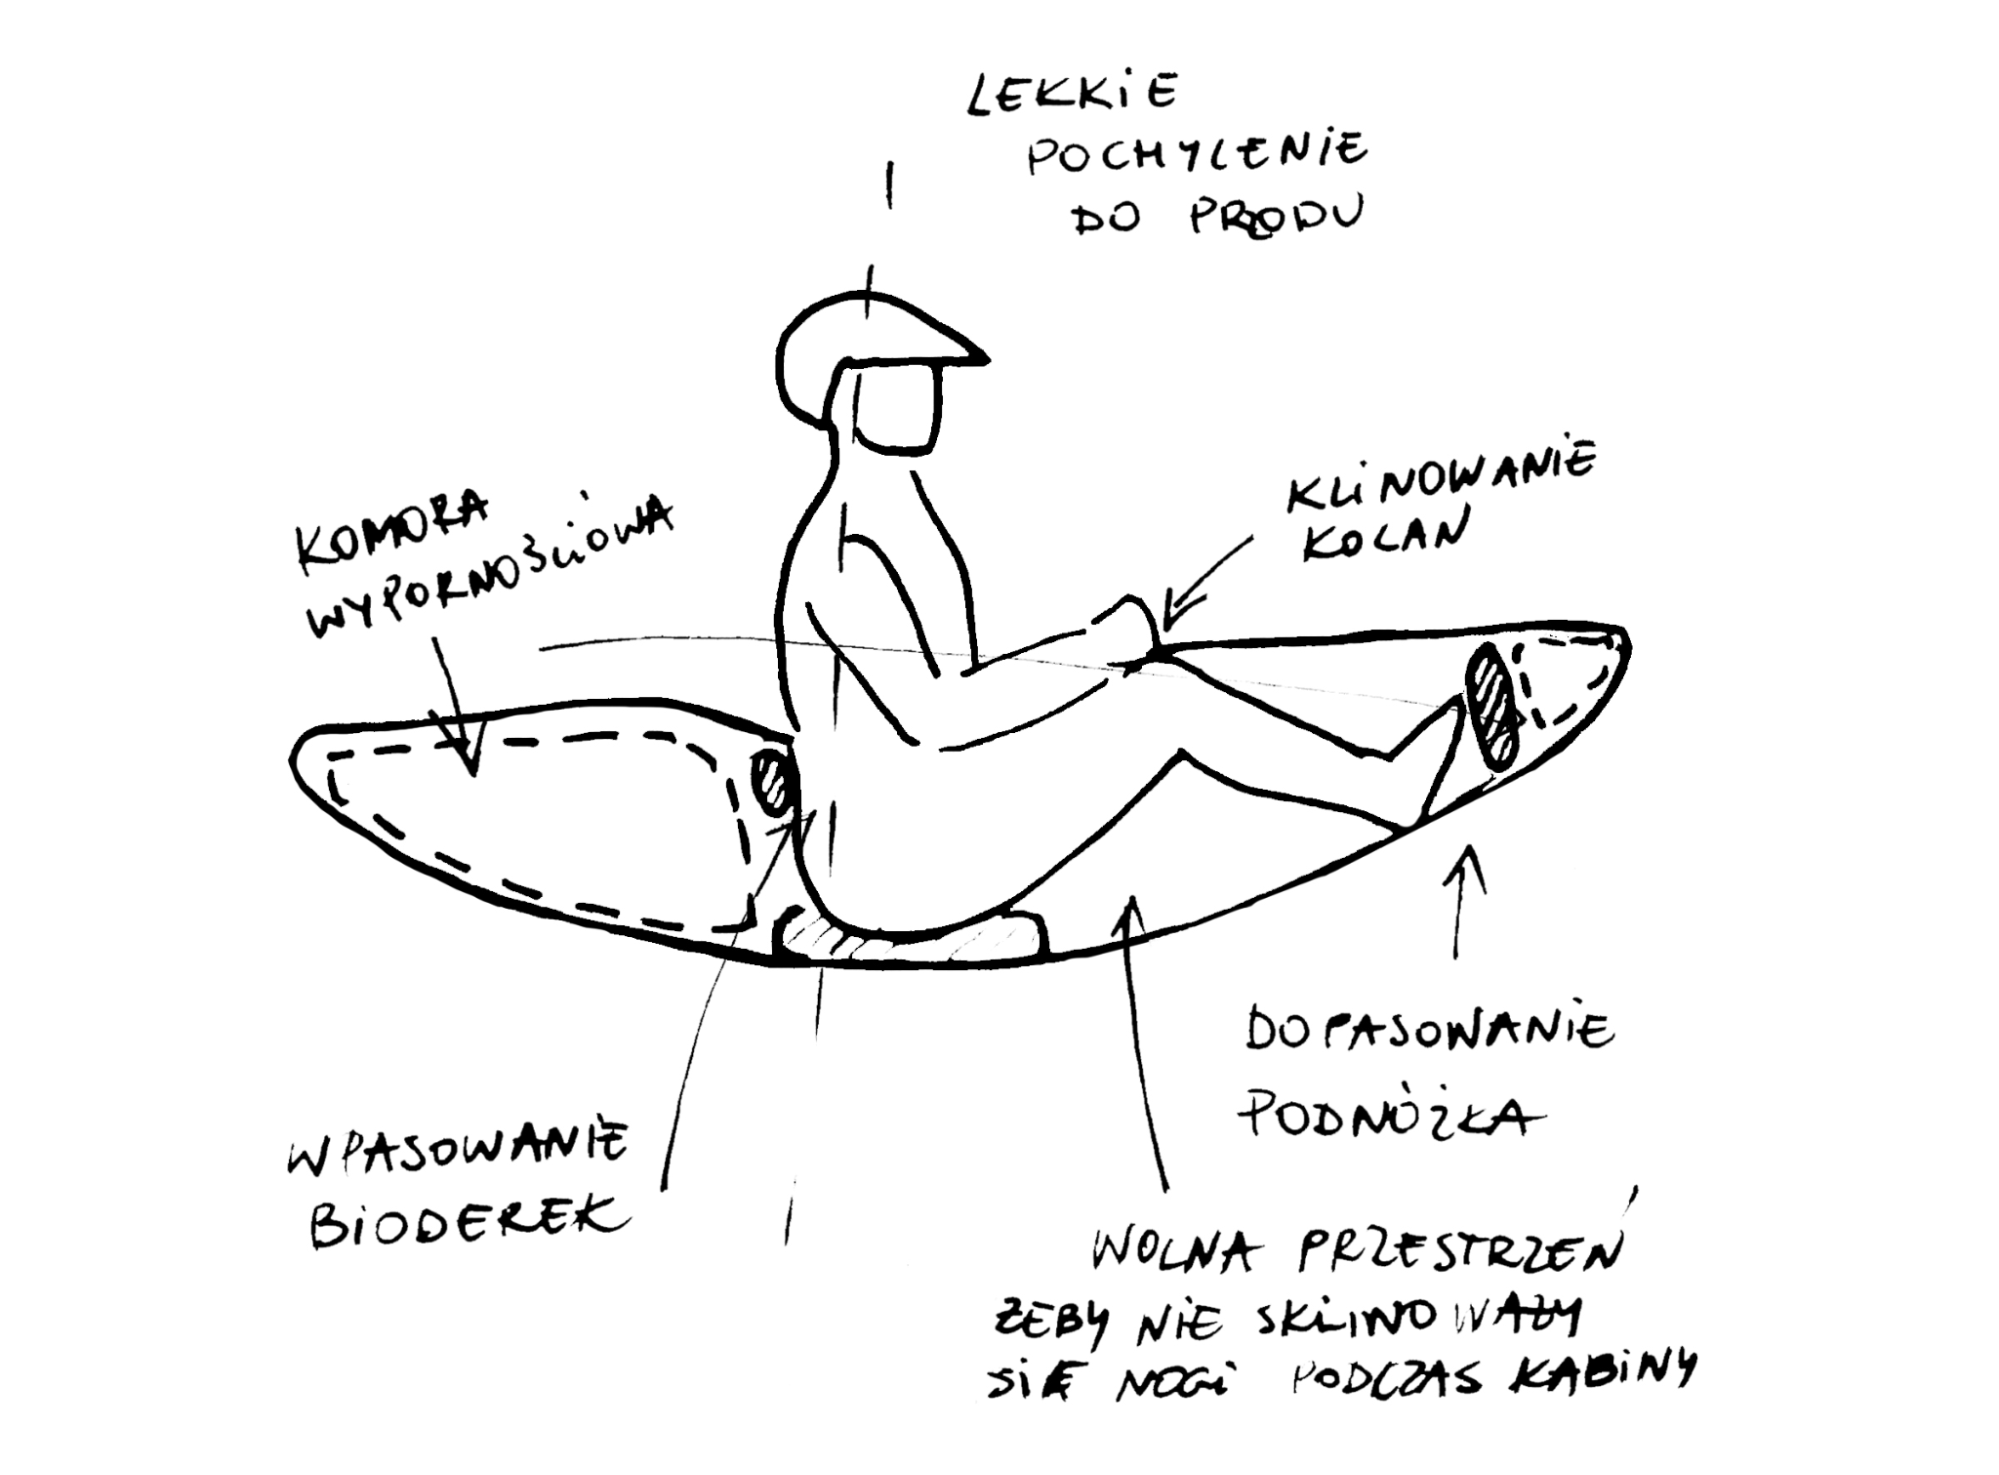
\includegraphics[width=300px]{images/pozycja_w_kajaku.png}
    \caption{Pozycja w kajaku}
\end{figure}

Oparcie służy do wsparcia pozycji na lędźwiach, ale nie opieramy się o nie całym ciężarem; w pozycji aktywnej oparcie powinno dotykać tylko pleców, nie naciskać na nie. Kolana oparte o \emph{motylki} (nakolanniki na burtach) pomagają sterować kajakiem. Biodra powinny mieścić się w siedzeniu i być z obu stron podparte boczkami przylegającymi całą powierzchnią do bioder. Pozycja powinna być neutralna — ciasno, ale komfortowo. Kolana wciskamy w górę w motylki, co daje większą kontrolę nad łódką. Drętwienie nóg i innych części ciała nie jest pożądane.

\begin{tipbox}
  \textbf{Safety box.} Trzymając wiosło, staraj się, aby kąty proste powstałe w łokciach i w obręczy barkowej utrzymywały się podczas manewrów — należy je wykonywać, balansując całą górną częścią ciała, a nie tylko zgięciem w łokciu. Wyobraź sobie, że przed sobą trzymasz pudło i razem z nim poruszasz tułowiem. Taka pozycja stabilizuje obręcz barkową i zabezpiecza przed zwichnięciem oraz wybiciem barków.
\end{tipbox}

\begin{figure}[h]
    \centering
    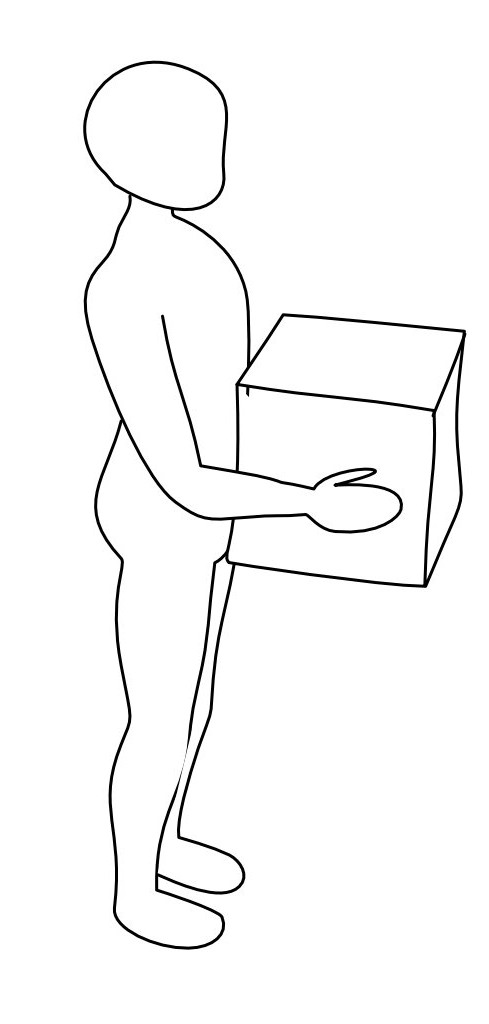
\includegraphics[width=100px]{images/safety_box.jpg}
    \caption{Wizualizacja zasady safety box}
\end{figure}


% ------------------------------------------------------------
\subsection{Rodzaje kajaków}
% ------------------------------------------------------------

Jest wiele rodzajów kajaków (m.in.\ nizinne/zwałkowe, packrafty, slalom, kanadyjki i inne), jednak skupmy się na tych, które będą nas głównie interesować jako kajakarzy pływających docelowo po górach i torach kajakowych.

\begin{description}[leftmargin=1.5em, style=nextline, font=\bfseries]

  \item[Creek]
    Kajak do trudnych, stromych rzek górskich. Duża wyporność, zaokrąglony dziób i rufa. Bardzo stabilny, bezpieczny przy wodospadach i progach. Przeznaczony na trudniejsze odcinki.

  \item[River runner]
    Kajak do stromych rzek górskich. Duża wyporność, zaokrąglony dziób i rufa. Szybszy, ale mniej stabilny od typowego creeka.

  \item[Half-slice]
    Kajak pośredni między river runnerem a playboatem. Posiada okrągły dziób z rockerem (zadartym noskiem), ale cienką rufę. Pozwala na triki i zabawę, ale nadal nadaje się na spływy górskie. Popularny wśród zaawansowanych kajakarzy.

  \item[Playboat / Freestyle]
    Kajak do trików i zabawy w falach oraz odwojach. Krótki i bardzo zwrotny, o małej wyporności, często z płaskim dnem. Raczej nie nadaje się do pływania w górach;na torze kajakowym może się sprawdzić. Nie nadaje się na długie spływy.

  \item[Full-slice]
    Kajak o małej wyporności na całej długości. Bardzo reaktywny i techniczny — idealny do freestyle'u i zabawy. Wymaga dużych umiejętności.

\end{description}

\subsubsection*{Kryteria doboru kajaka}

\begin{description}[leftmargin=1.5em, font=\bfseries]
  \item[Cel]
    Dobieramy kajak odpowiednio do swoich umiejętności, poziomu trudności akwenu i elementów, które będziemy ćwiczyć. Inny kajak wybierzemy na trudną rzekę górską, inny na tor kajakowy, a jeszcze inny na płaską wodę.

  \item[Waga kajakarza]
    Warto stosować się do zakresu wagowego kajaka — ma to wpływ na bezpieczeństwo, zanurzenie łódki, wyporność i stabilność. Przekroczenie wagi prowadzi do utraty stabilności i zwiększa ryzyko wywrotki; zbyt duży kajak jest mniej sterowny i wymaga więcej siły. Wybór zbyt dużego kajaka utrudnia też naukę i oswajanie się
    z wywrotkami.
\end{description}

% ------------------------------------------------------------
\subsection{Wiosło}
% ------------------------------------------------------------

Wiosło składa się z \textbf{dwóch piór} (strona pasywna — wypukła; strona aktywna — wklęsła) oraz \textbf{drążka}.

\textbf{Długość.}
Odpowiednia długość wiosła odpowiada mniej więcej wysokości nadgarstka kajakarza z ręką wyciągniętą do góry (z uwzględnieniem indywidualnych preferencji). Im dłuższe wiosło, tym trudniejsze może być wiosłowanie; jednak dla wysokich osób lub szerokiego kajaka jest ono wskazane. Krótszym wiosłem można wiosłować bardziej agresywnie i pionowo.

\begin{figure}[h]
    \centering
    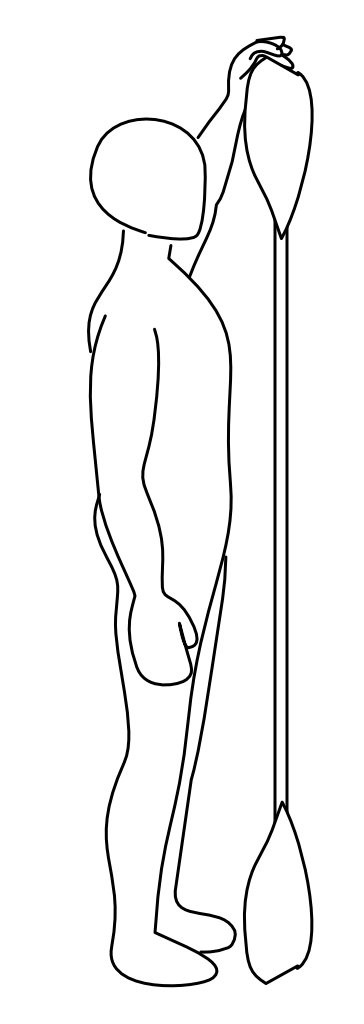
\includegraphics[width=80px]{images/dlugosc_wiosla.jpg}
    \caption{Przyklad metody dobioru dlugości wiosła}
\end{figure}

\textbf{Rotacja pióra.}
Zapewnia komfort i efektywność podczas wiosłowania. Przy wiosłach skrętnych ruch nadgarstków jest bardziej ergonomiczny, co pomaga podczas dłuższych spływów. W kajakarstwie górskim najczęściej spotykane są kąty w okolicach 30-45°. Wiosła proste są głównie wykorzystywane we freestyle'u, gdzie symetria ruchów po obu stronach jest kluczowa.

% ------------------------------------------------------------
\subsection{Fartuch}
% ------------------------------------------------------------

Komin fartucha nakładamy na ciało na wysokości pasa (może sięgać nawet do klatki piersiowej). Gumę na obwodzie zakłada się na kokpit kajaka — fartuch zapobiega wlewaniu się wody do kajaka. Dobrze dobrany fartuch powinniśmy móc samodzielnie założyć na kajak oraz zerwać go w przypadku konieczności szybkiego opuszczenia kajaka. 

Rozmiar \textbf{pokładu} fartucha musi być dopasowany do rozmiaru kokpitu kajaka, a rozmiar \textbf{komina} — do obwodu w pasie.

\begin{tipbox}
  Mokry neopren łatwiej się rozciąga — jeśli masz problem z naciągnięciem fartucha na kokpicie, zamocz fartuch przed założeniem.
\end{tipbox}

% ------------------------------------------------------------
\subsection{Kask}
% ------------------------------------------------------------

Kask powinien być dobrze dopasowany do głowy — nie poruszać się przy potrząsaniu głową, nawet gdy jesteśmy pochyleni. Chroni przed stłuczeniami i urazami spowodowanymi uderzeniem o skałę, wiosło współtowarzyszy lub krawędź basenu.

Pasek zapinamy \textbf{zawsze} — nawet na lądzie. Wyrobieniu tego nawyku służy konsekwentne zapinanie kasku poza wodą. Pasek powinien być ciasny, ale nie utrudniać oddychania.

\begin{tipbox}
  Każda firma ma własny zakres rozmiarów, który nie gwarantuje idealnego dopasowania. Przed wyjazdem warto przymierzyć kask klubowy, a przed zakupem własnego pożyczyć go na próbę od znajomych.
\end{tipbox}

% ------------------------------------------------------------
\subsection{Kamizelka}
% ------------------------------------------------------------

\textbf{Kamizelki górskie} mają dużą wyporność pozwalającą na utrzymanie kajakarza na powierzchni rwącej wody. Mają wbudowany pas przystosowany do wpięcia podczas akcji ratunkowej (z możliwością szybkiego wypięcia), liczne kieszenie i uchwyty. Pomimo rozbudowanej konstrukcji zapewniają dużą swobodę ruchów.

Na rzekach nizinnych wystarczająca jest \textbf{kamizelka nizinna} — mniej wyporna, ale ze względu na prostszą konstrukcję mniej ograniczająca ruchy przy pokonywaniu zwałek.

% ------------------------------------------------------------
\subsection{Rzutka}
% ------------------------------------------------------------

Miękka, mocna lina o jaskrawym kolorze, unosząca się na wodzie, znajdująca się w worku. Główne zastosowanie: rzucanie w celu wyłowienia osoby znajdującej się w wodzie. Dostępna w długościach 10-35\,m (dobieramy w zależności od potrzeb i umiejętności rzucającego). Rzutka powinna być zawsze dobrze \textbf{sklarowana} (ułożona w worku).
i gotowa do użycia.

\begin{warnbox}
  Na rzece górskiej należy \textbf{ZAWSZE} mieć rzutkę przy sobie — nawet gdy wychodzimy z kajaka obserwując rzekę z brzegu. Używając liny, zawsze warto mieć przy sobie \textbf{nóż}.
\end{warnbox}

% ------------------------------------------------------------
\subsection{Komory}
% ------------------------------------------------------------

Komory służą do wypełnienia kajaka powietrzem. Nie poprawiają wyporności kajaka, natomiast dzięki nim kajak nabiera mniejszą ilość wody po kabinie, co znacznie ułatwia jego wyłowienie.

Komory występują zazwyczaj w rozmiarach:

\begin{itemize}[leftmargin=1.5em]
  \item \textbf{20\,L} — wsadza się na tył kajaka (zazwyczaj dwie, jeśli przez środekprzebiega przegroda)
  \item \textbf{10\,L} — wsadza się na przód kajaka, jeśli za podnóżkiem jest miejsce
\end{itemize}

% ------------------------------------------------------------
\subsection{Ubiór kajakarza i lista rzeczy na spływ}
% ------------------------------------------------------------

\begin{tabular}{>{\bfseries}p{3cm} p{10cm}}
\toprule
\textbf{Kategoria} & \textbf{Wyposażenie} \\
\midrule

Basen &
\begin{itemize}[leftmargin=*, nosep, topsep=0pt]
  \item Kąpielówki przylegające
  \item Nosek
  \item Zatyczki do uszu*
  \item Klapki
  \item Okularki (opcjonalnie)
  \item Ręcznik
\end{itemize} \\
\midrule

Pływanie &
\begin{itemize}[leftmargin=*, nosep, topsep=0pt]
  \item Obuwie do wody / neoprenowe (wiązane, grubsza podeszwa)
  \item Czapka z daszkiem / kapelusz / bandana
  \item Krem z filtrem
  \item Bidon
  \item Wodoodporny worek z suchymi ubraniami
  \item Nosek, zatyczki do uszu (opcjonalne)
  \item Ubranie dopasowane do pogody (neopren / polar / kurtka pół-sucha lub sucha)
\end{itemize} \\
\midrule

Biwak &
\begin{itemize}[leftmargin=*, nosep, topsep=0pt]
  \item Namiot
  \item Karimata
  \item Śpiwór
  \item Odzież: polar, neopren lub wełna
  \item Ciepłe nakrycie głowy
  \item Płaszcz przeciwdeszczowy
  \item Latarka / czołówka
  \item Menażka, kubek, sztućce
  \item Spray na komary
  \item \textbf{Dobry humor :)}
\end{itemize} \\
\midrule

Dodatkowo &
\begin{itemize}[leftmargin=*, nosep, topsep=0pt]
  \item Krem z filtrem
  \item Pomadka nawilżająca
  \item Krzesełko turystyczne
  \item Instrument muzyczny
  \item Nóż składany
  \item Apteczka
  \item Taśma z karabinkiem
  \item Bidon z wodą
\end{itemize} \\
\bottomrule
\end{tabular}
% ============================================================
%  Rozdział 3 — Locja
% ============================================================
\section{Locja}

% ------------------------------------------------------------
\subsection{Skala oceny trudności}
% ------------------------------------------------------------

\begin{longtable}{>{\bfseries\centering}p{1.8cm}
                  >{\centering}p{2.2cm}
                  p{5.2cm}
                  p{4.2cm}}
  \toprule
  \textbf{Stopień WW} & \textbf{Nazwa} & \textbf{Charakterystyka rzeki}
    & \textbf{Wymagania dla kajakarza} \\
  \midrule
  \endfirsthead
  \toprule
  \textbf{Stopień WW} & \textbf{Nazwa} & \textbf{Charakterystyka rzeki}
    & \textbf{Wymagania dla kajakarza} \\
  \midrule
  \endhead
  \bottomrule
  \endfoot

  WW I & Bardzo łatwa
    & Nurt szybki, ale czytelny; drobne fale; brak istotnych przeszkód. & Podstawowe umiejętności sterowania. \\[4pt]

  WW II & Łatwa & Wyraźne bystrza, małe fale, proste przeszkody; dobra widoczność linii. & Kontrola kajaka, podstawowa technika. \\[4pt]

  WW III & Średnia & Silniejszy nurt, większe fale, progi, odwoje; wymagane manewry. & Dobra technika, pewna eskimoska; linia płynięcia możliwa do odczytania
      z kajaka. \\[4pt]

  WW IV & Trudna & Długie, techniczne bystrza, silne odwoje, ciasne linie. & Bardzo dobra technika, czytanie wody; miejscami konieczne planowanie linii z brzegu; ryzyko kontuzji przy odejściu od zaplanowanej linii. \\[4pt]

  WW V & Bardzo trudna & Duże spadki, wodospady, groźne odwoje i podmycia. & Ekspercka technika, asekuracja, skautowanie z brzegu; odejście od linii niesie ryzyko poważnej kontuzji lub śmierci. \\[4pt]

  WW VI & Ekstremalna & Skrajnie niebezpieczna, praktycznie niepływalna. & Ekspedycje ekstremalne, wielodniowe skautowanie; wysokie ryzyko śmierci. \\
\end{longtable}

% ------------------------------------------------------------
\subsection{Brzeg}
% ------------------------------------------------------------

Krawędź koryta rzeki. Oddziela wodę płynącą od lądu i jest kształtowany przez nurt. Brzeg może być \textbf{prawy} lub \textbf{lewy} — określamy je patrząc \emph{w dół rzeki},
z nurtem. Takie podejście niweluje nieporozumienia w komunikacji kajakarzy. Brzeg bywa miejscem zagrożeń, dlatego nawet znajdując się na nim konieczne jest zachowanie szczególnej ostrożności.

% ------------------------------------------------------------
\subsection{Nurt}
% ------------------------------------------------------------

Kierunek i ruch wody w rzece. Jego siłę i kierunek determinuje ilość wody, kierunek, spadek terenu oraz różne przeszkody w korycie.

% ------------------------------------------------------------
\subsection{Bystrze}
% ------------------------------------------------------------

Odcinek rzeki, na którym następuje przyspieszenie nurtu spowodowane wypłyceniem, zwężeniem, spadkiem terenu lub innymi czynnikami. Woda jest wzburzona, nurt rozbija się o kamienie tworząc fale, białe grzywy i prądy. Bystrza zawierają takie elementy jak głazy, cofki, hyżki, odwoje, podmytki, poduszki.

Upraszczając, mają kształt litery „V" rozwartej w górę rzeki — jeśli nie ma większych przeszkód, najlepiej płynąć środkiem.

% ------------------------------------------------------------
\subsection{Zwałka}
% ------------------------------------------------------------

Przeszkoda na rzece do pokonania nad nią lub pod (czasami bez konieczności wysiadania z kajaka). Przykład: przewrócone drzewo.

% ------------------------------------------------------------
\subsection{Cofka}
% ------------------------------------------------------------

Miejsce na rzece z nurtem przeciwnym do głównego nurtu rzeki, często dużo wolniejszym i spokojniejszym. Tworzy się za przeszkodą — kamieniem, gałęzią, drzewem, mielizną, zakrętem itp. Może powstawać przy brzegu lub na środku rzeki.

Jest \textbf{bardzo ważnym elementem rzeki} dla kajakarza — pełni rolę miejsca do wsiadania lub bezpiecznego opuszczenia kajaka, odpoczynku, rozejrzenia się, obejrzenia dalszego
odcinka, zaplanowania trasy i zebrania grupy.

Nie każda cofka jest bezpieczna — zawsze oceniamy ją samodzielnie. Na co zwrócić uwagę: 

\begin{itemize}[leftmargin=1.5em, itemsep=3pt]
  \item \textbf{Długość cofki} — zbyt krótka może być trudna do złapania lub może wymyć kajakarza, zmuszając go do dalszego płynięcia. 
  \item \textbf{Szerokość cofki} — dobrze, jeśli jest przynajmniej tak szeroka, że kajak obróci się w niej w osi poziomej o 360°.
  \item \textbf{Pulsacja wody} — gdy woda pulsuje, zmienia się jej poziom w cofce i trudniej jest się w niej utrzymać; czasem cofka może zniknąć i po chwili pojawić się ponownie.
\end{itemize}

% ------------------------------------------------------------
\subsection{Hyżka}
% ------------------------------------------------------------

Granica między głównym nurtem a cofką. Na samym początku (zaraz za przeszkodą) jest wąska, ale rozszerza się i rozmywa w dół głównego nurtu. Wchodząc do cofki, kajakarzowi zależy
na przecięciu hyżki z odpowiednią prędkością, jak najwyżej / jak najbliżej przeszkody, która tę cofkę tworzy.

\begin{figure}[H]
    \centering
    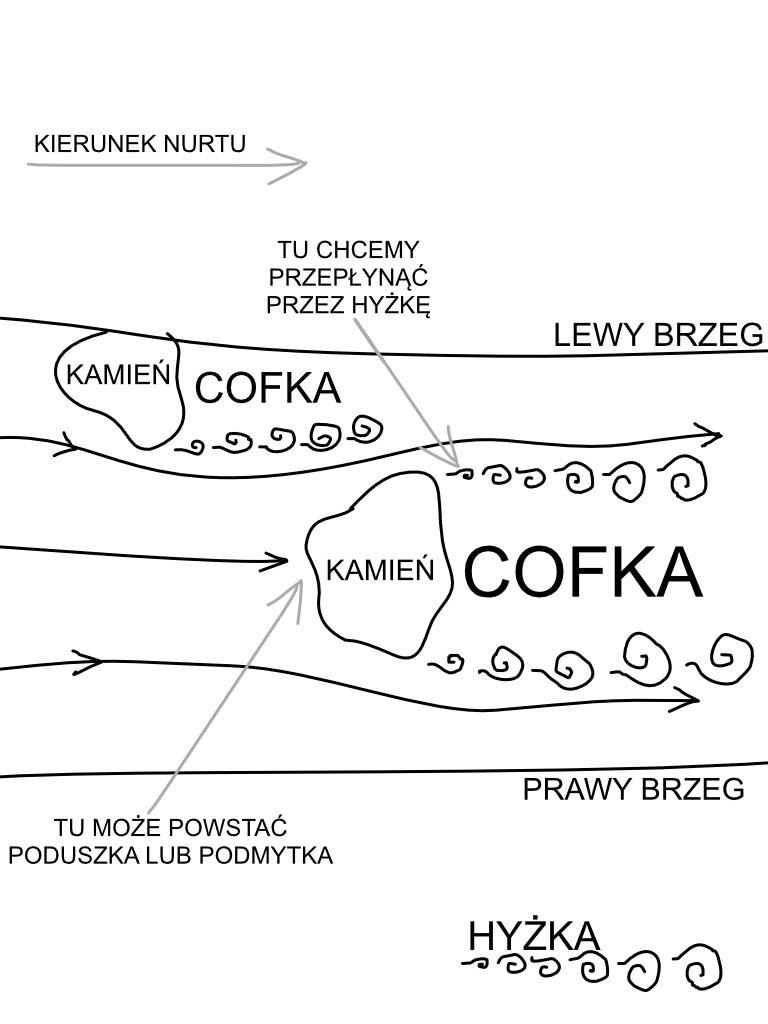
\includegraphics[width=250px]{images/locja.jpg}
    \caption{Opis wybranych elementów rzeki}
\end{figure}

% ------------------------------------------------------------
\subsection{Odwój}
% ------------------------------------------------------------

Element rzeki powstający poniżej progu, stopnia lub przeszkody, gdzie spadająca woda cofa się w górę rzeki tworząc „wałek" spowalniający. Woda spadająca z progu uderza w taflę lub dno, zawijając się w górę i w kierunku progu.

\subsubsection*{Płytka cyrkulacja}

Wałek, w którym obieg wody zachodzi głównie przy powierzchni. Woda miesza się dynamicznie, ale szybko „puszcza" kajak lub pływaka, wypychając go do przodu. Najczęściej występuje
na naturalnych bystrzach i małych progach. Fala jest głośna, spieniona i wyraźna. Zagrożenie niskie do umiarkowanego; możliwość samodzielnego wypłynięcia duża. \emph{Strategia: zdecydowane przepłynięcie z prędkością.}

\subsubsection*{Głęboka cyrkulacja}

Niebezpieczny wałek z głębokim, zamkniętym obiegiem wody. Silnie wciąga w stronę dna i może wielokrotnie „prać" pływaka, utrudniając wydostanie się. Często występuje poniżej
sztucznych progów i zapór. Fala bywa regularna i pozornie spokojna. Zagrożenie wysokie; możliwość samodzielnego wypłynięcia bardzo mała. \emph{Strategia: omijanie lub przenoska.}

\vspace{0.5em}
\noindent
\begin{minipage}[t]{0.48\linewidth}
\begin{tcolorbox}[
  equal height group=odwoj,
  colback=clubgray, colframe=clubblue!60,
  fonttitle=\bfseries\color{white},
  title=Płytka cyrkulacja,
  coltitle=white, colbacktitle=clubblue!60
]
\begin{description}[leftmargin=0pt, labelwidth=\linewidth, font=\bfseries\small]
  \item[Głębokość obiegu:] Głównie przy powierzchni
  \item[Kierunek sił:] Miesza wodę, szybko puszcza
  \item[Zachowanie wody:] Szybko wypycha do przodu
  \item[Wpływ na pływaka:] Chwilowe zatrzymanie
  \item[Możliwość wypłynięcia:] Duża
  \item[Typowe miejsce:] Naturalne bystrza, małe progi
  \item[Charakter fali:] Głośna, spieniona
  \item[Stopień zagrożenia:] Niski–umiarkowany
  \item[Strategia:] Przepłynięcie z prędkością
\end{description}
\end{tcolorbox}
\end{minipage}
\hfill
\begin{minipage}[t]{0.48\linewidth}
\begin{tcolorbox}[
  equal height group=odwoj,
  colback=warnred, colframe=warnframe,
  fonttitle=\bfseries,
  title=Głęboka cyrkulacja,
  coltitle=white, colbacktitle=warnframe
]
\begin{description}[leftmargin=0pt, labelwidth=\linewidth, font=\bfseries\small]
  \item[Głębokość obiegu:] Sięga głęboko pod wodę
  \item[Kierunek sił:] Silne wciąganie w stronę dna
  \item[Zachowanie wody:] Krąży w zamkniętej pętli
  \item[Wpływ na pływaka:] Wielokrotne "pranie"; wciąganie pod wodę
  \item[Możliwość wypłynięcia:] Bardzo mała
  \item[Typowe miejsce:] Sztuczne progi, zapory
  \item[Charakter fali:] Regularna, cicha, bez widocznej grzywy
  \item[Stopień zagrożenia:] Wysoki / śmiertelny
  \item[Strategia:] Omijanie, przenoska
\end{description}
\end{tcolorbox}
\end{minipage}
\vspace{0.5em}

\begin{figure}[H]
  \centering
  \begin{minipage}[t]{0.48\linewidth}
    \centering
    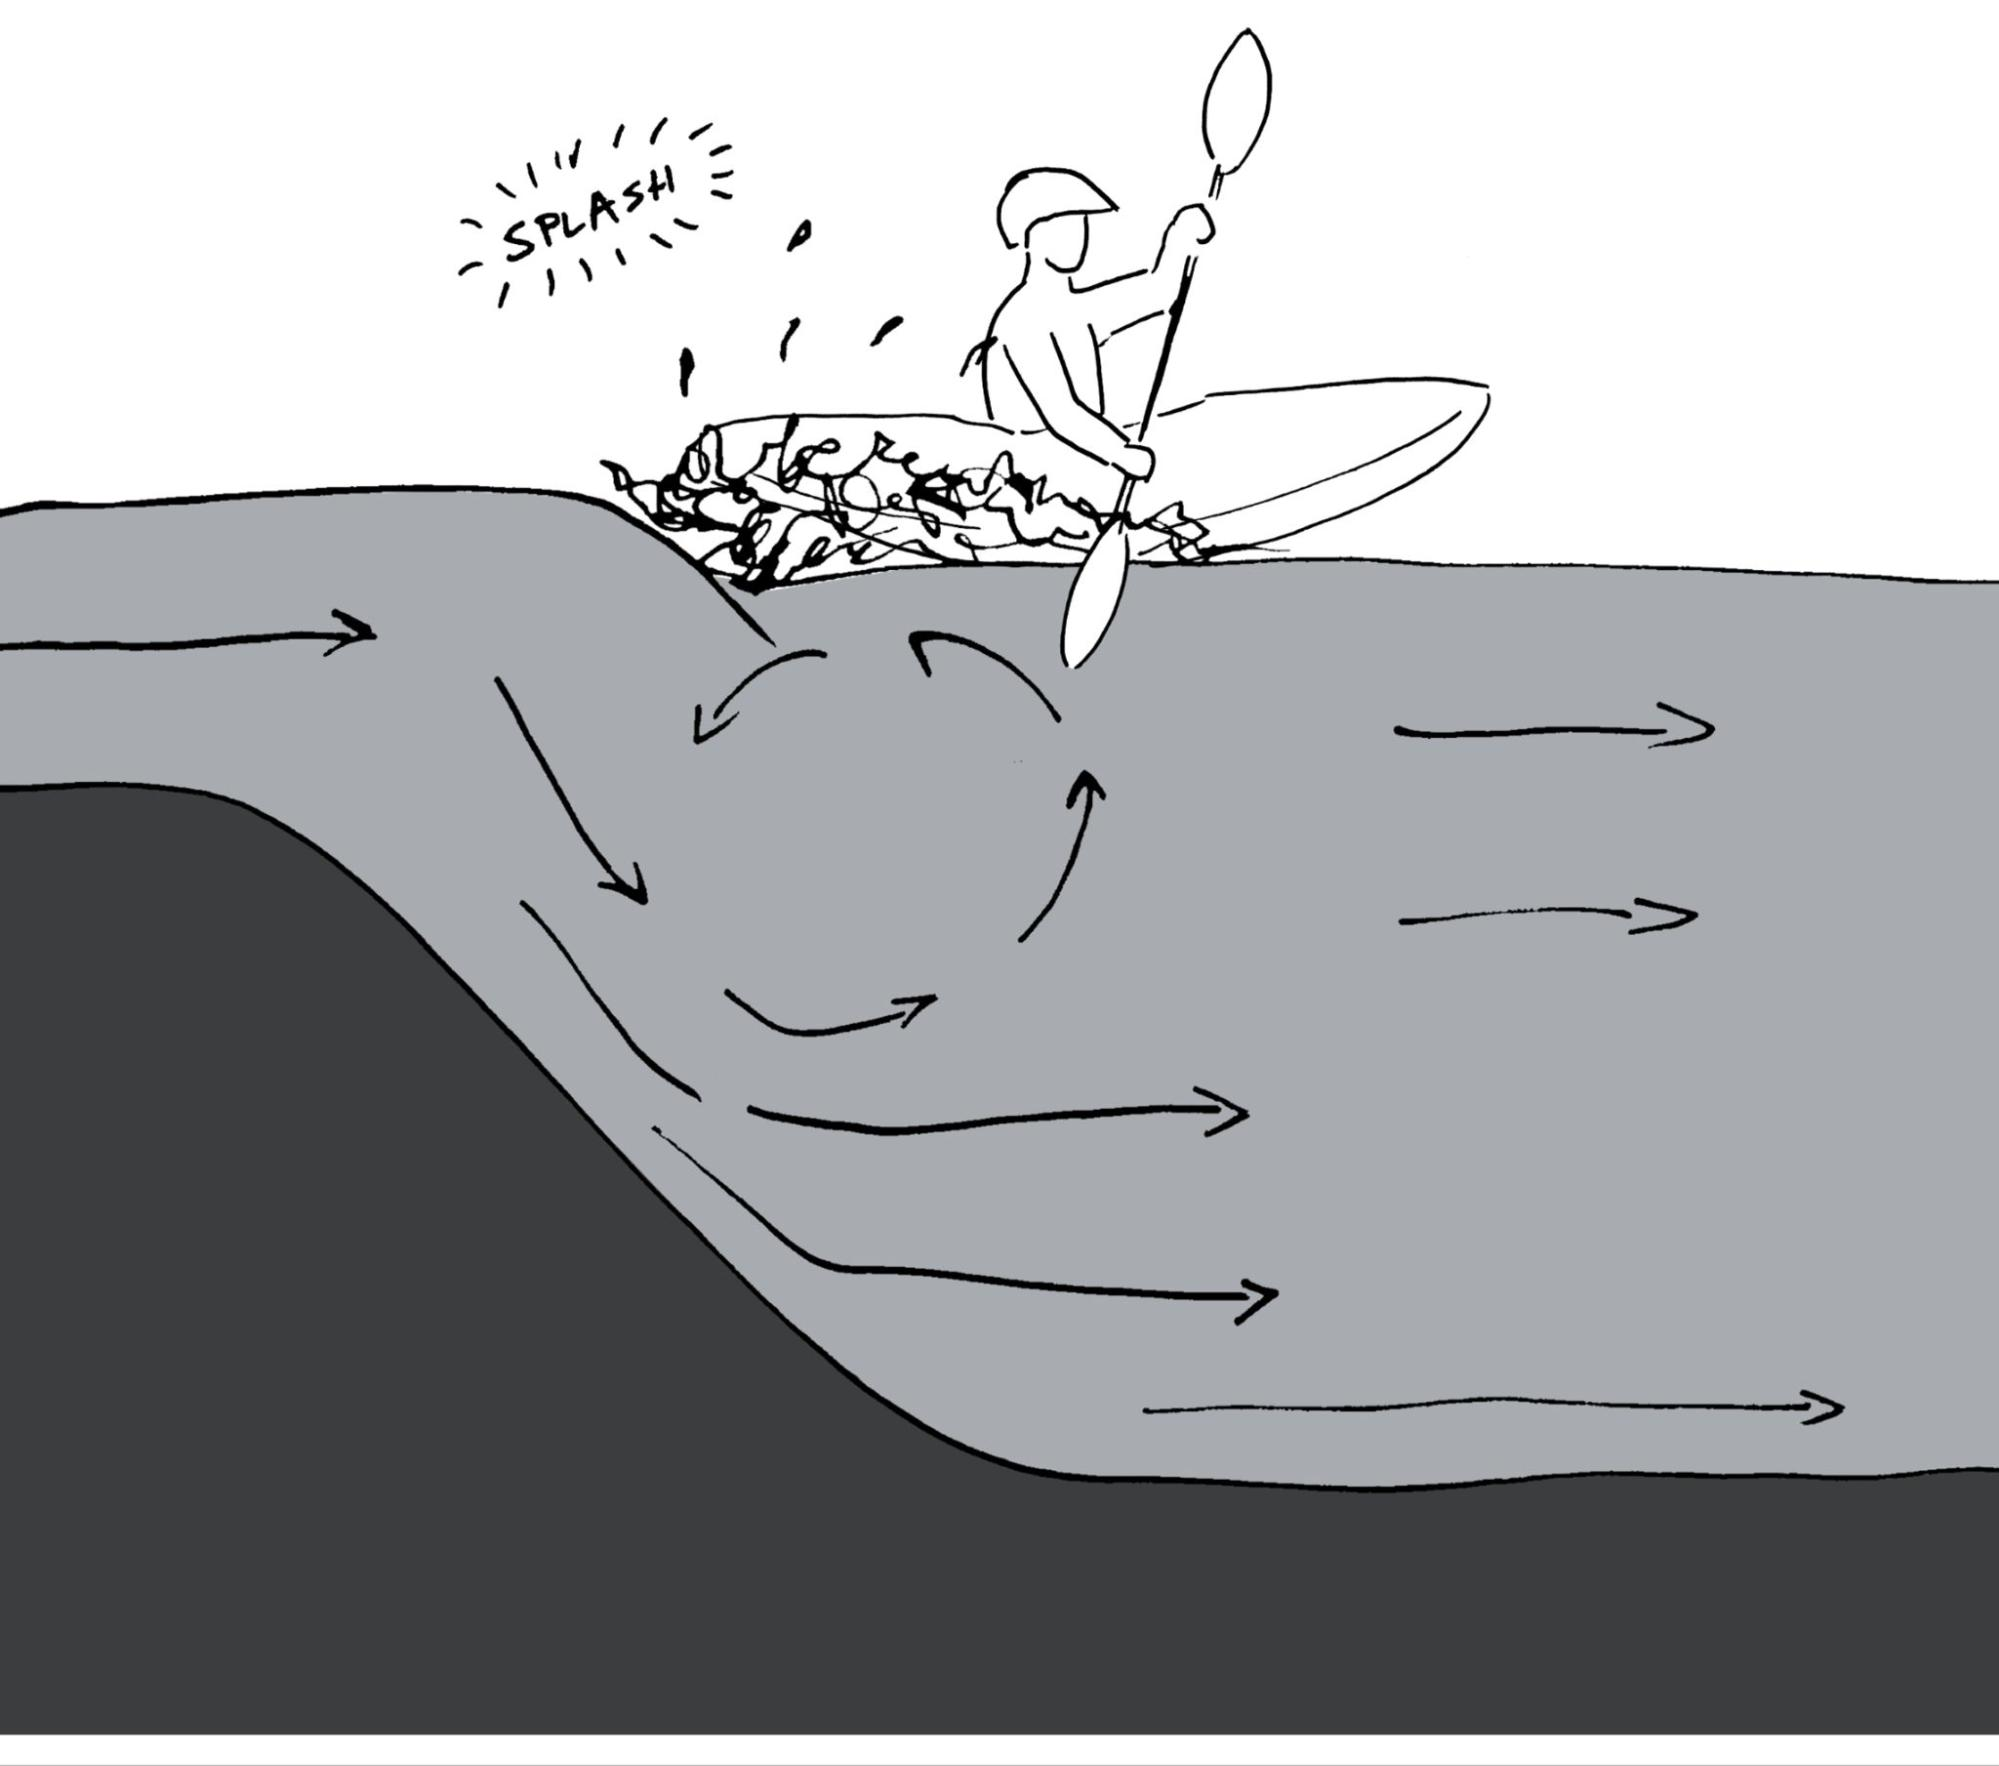
\includegraphics[width=\linewidth]{images/plytki_odwoj.jpg}
    \caption*{(a) Odwój o płytkiej cyrkulacji}
  \end{minipage}
  \hfill
  \begin{minipage}[t]{0.48\linewidth}
    \centering
    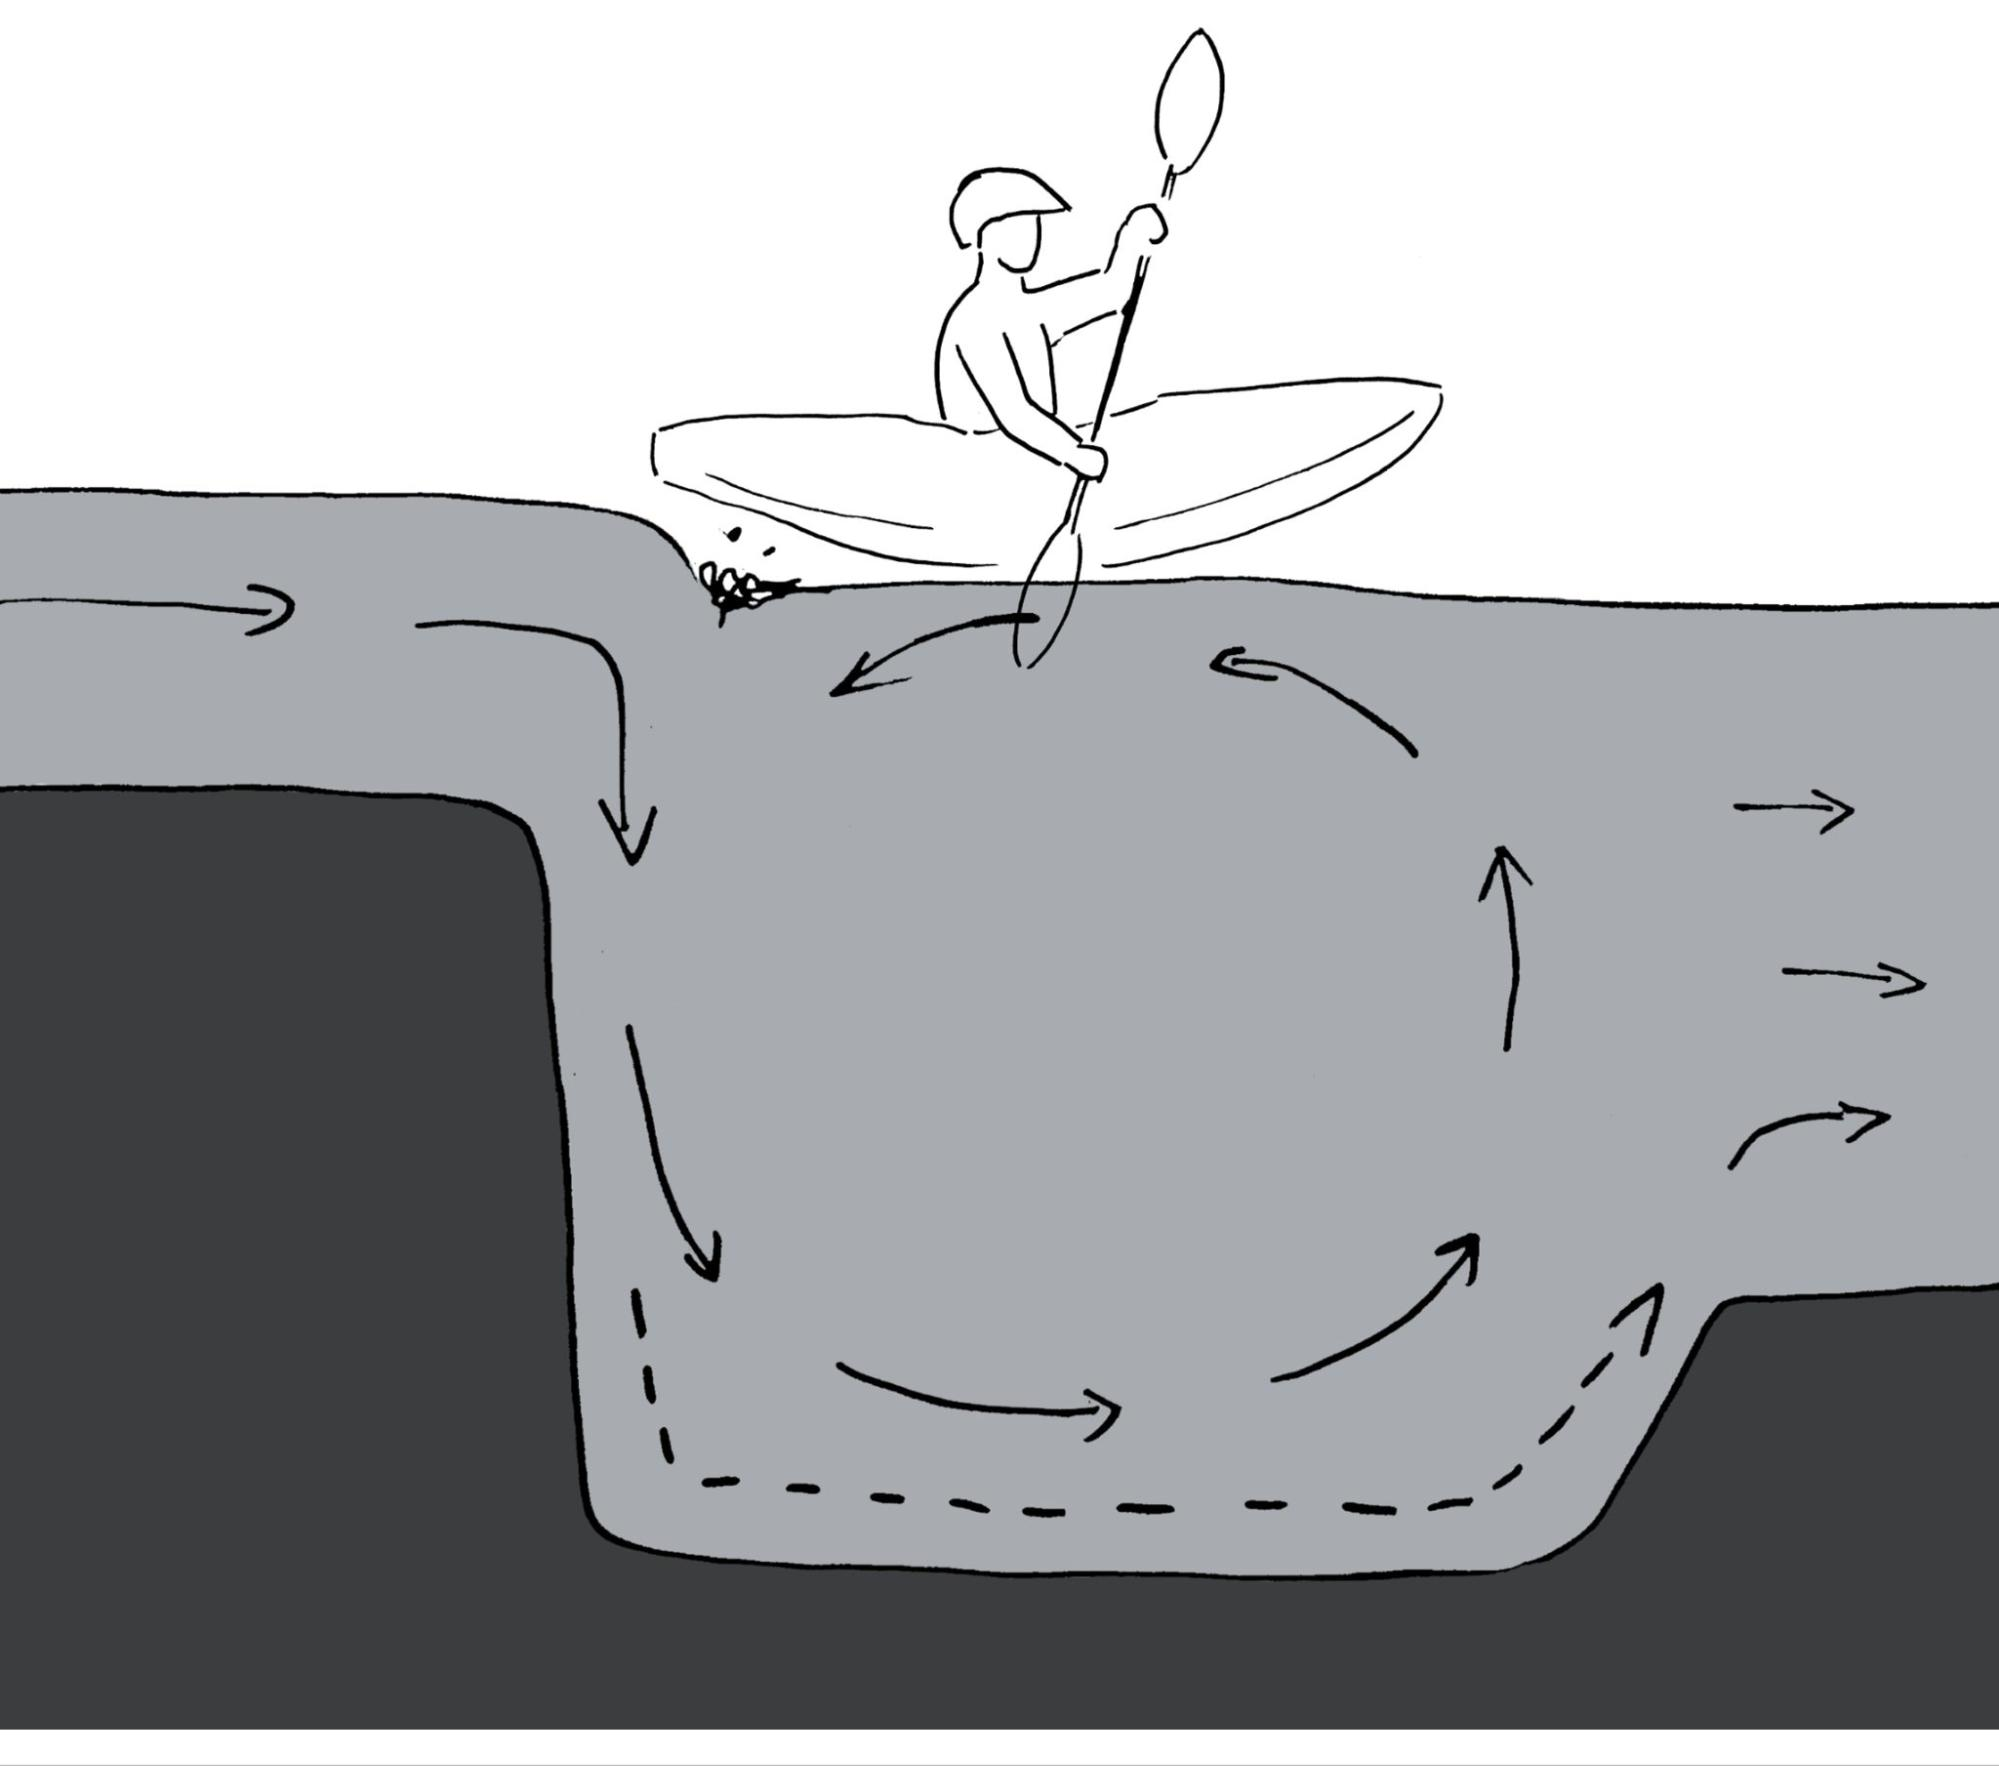
\includegraphics[width=\linewidth]{images/gleboki_odwoj.jpg}
    \caption*{(b) Odwój o głębokiej cyrkulacji}
  \end{minipage}
  \caption{Rodzaje odwojów}
\end{figure}

% ------------------------------------------------------------
\subsection{Podmytka / Syfon}
% ------------------------------------------------------------

Bardzo groźne miejsca na rzece górskiej. Podmytka to przeszkoda (najczęściej kamień, brzeg lub drzewo), pod którą woda przepływa swobodnie, jednak kajakarz może zostać wciągnięty pod nią przez nurt i przyparty do niej bez możliwości przedostania się na drugą stronę ze względu na swoje rozmiary. Podmytka różni się od syfonu tym, że jest z jednej strony otwarta; syfon to miejsce, gdzie nurt przepływa przez otwór w kamieniu bądź między narzuconymi kamieniami.

\begin{figure}[H]
    \centering
    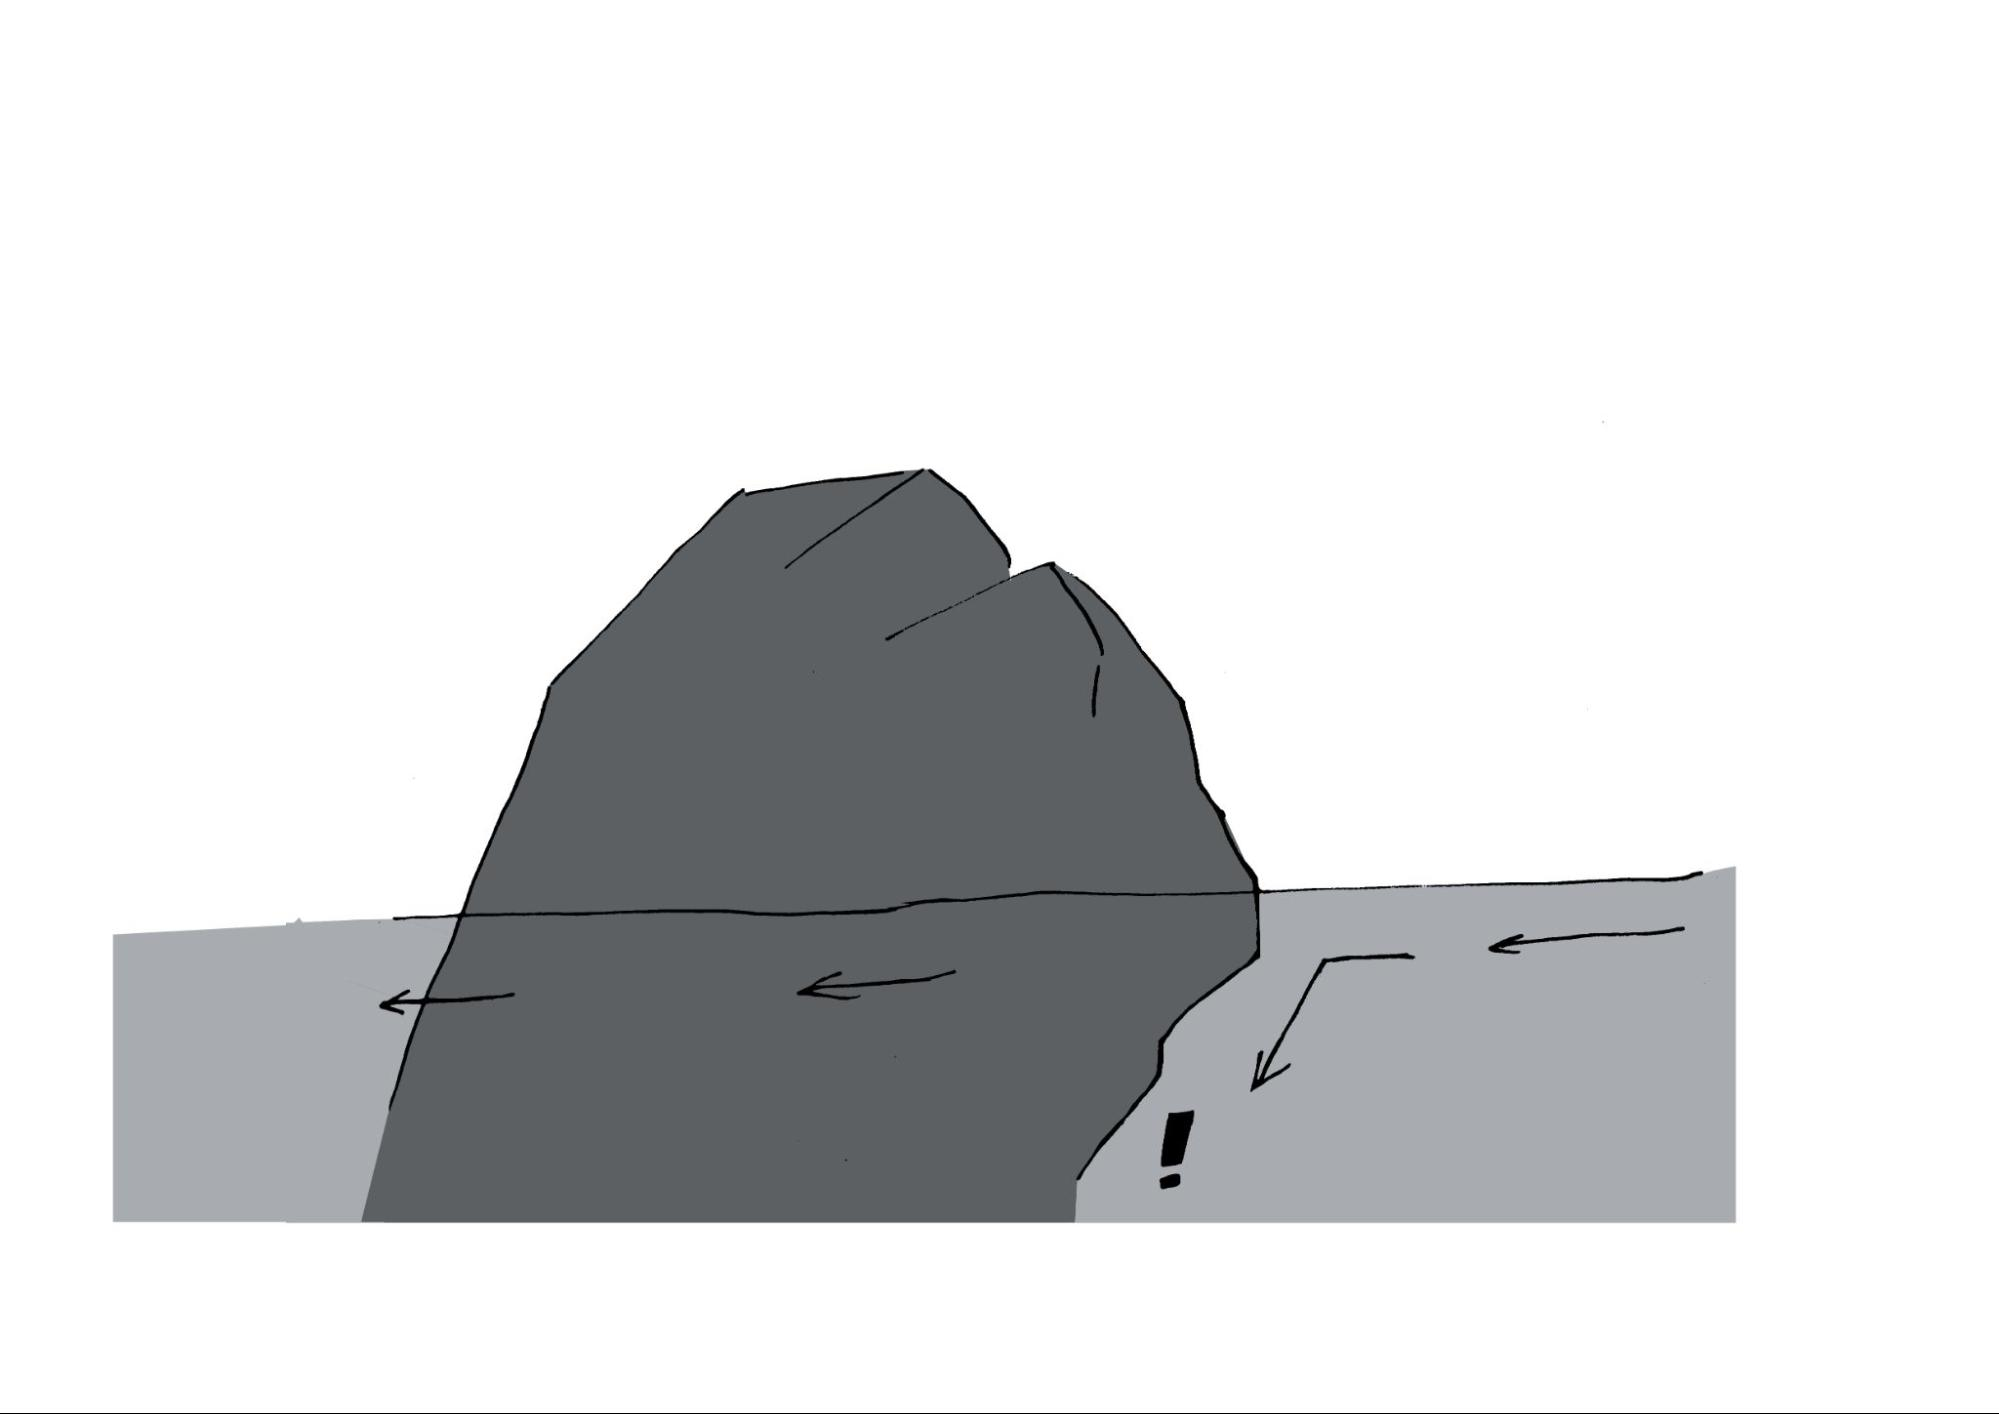
\includegraphics[width=300px]{images/podmytka_syfon.jpg}
    \caption{Wizualizacja podmytki / syfonu}
\end{figure}

\begin{warnbox}
  Podmytki i syfony należą do najbardziej niebezpiecznych przeszkód na rzece górskiej. Zawsze identyfikuj je z brzegu i bezwzględnie omijaj.
\end{warnbox}

% ------------------------------------------------------------
\subsection{Poduszka / Maliniak}
% ------------------------------------------------------------

\textbf{Maliniak} tworzy się, gdy woda wypływająca pionowo (od dna do powierzchni) tworzy charakterystyczny grzybek, na którym kajak może stracić stabilność.

\textbf{Poduszka} to sytuacja, gdzie woda odbija się od kamienia w nurcie — w ten sposób można bezpiecznie rozpoznać kamienie, które dostarczają wiele frajdy doświadczonym kajakarzom.
% ============================================================
%  Rozdział 4 — PKP: Prędkość, Kąt, Przechył
% ============================================================
\section{PKP — Prędkość, Kąt, Przechył}

Najbardziej istotne elementy przy większości manewrów — szczególnie przy wchodzeniu
i wychodzeniu z cofki — to \textbf{P}rędkość, \textbf{K}ąt i \textbf{P}rzechył.

\begin{description}[leftmargin=1.5em, style=nextline, font=\bfseries]

  \item[Prędkość]
    Pozwala na przecięcie hyżki. Bez odpowiedniej prędkości wyjście z cofki jest niemożliwe — hyżka zabiera dziób kajaka i obracamy się w miejscu.

  \item[Kąt]
    Pozycja kajaka w stosunku do hyżki. Pomaga lub utrudnia przecięcie hyżki i decyduje o tym, w jakiej pozycji kajak znajdzie się po wykonaniu manewru. Odpowiedni kąt zależy
    też od siły nurtu — im mocniejszy nurt, tym ostrzejszy kąt.

  \item[Przechył]
    Pomaga ustabilizować i kontrolować kajak. Powinien być mały, ale stabilny. Zasada: \textbf{DUPA DO NURTU} — nurt zawsze powinien napierać na krawędź znajdującą
    się wyżej, najlepiej w dno kajaka.

\begin{figure}[H]
    \centering
    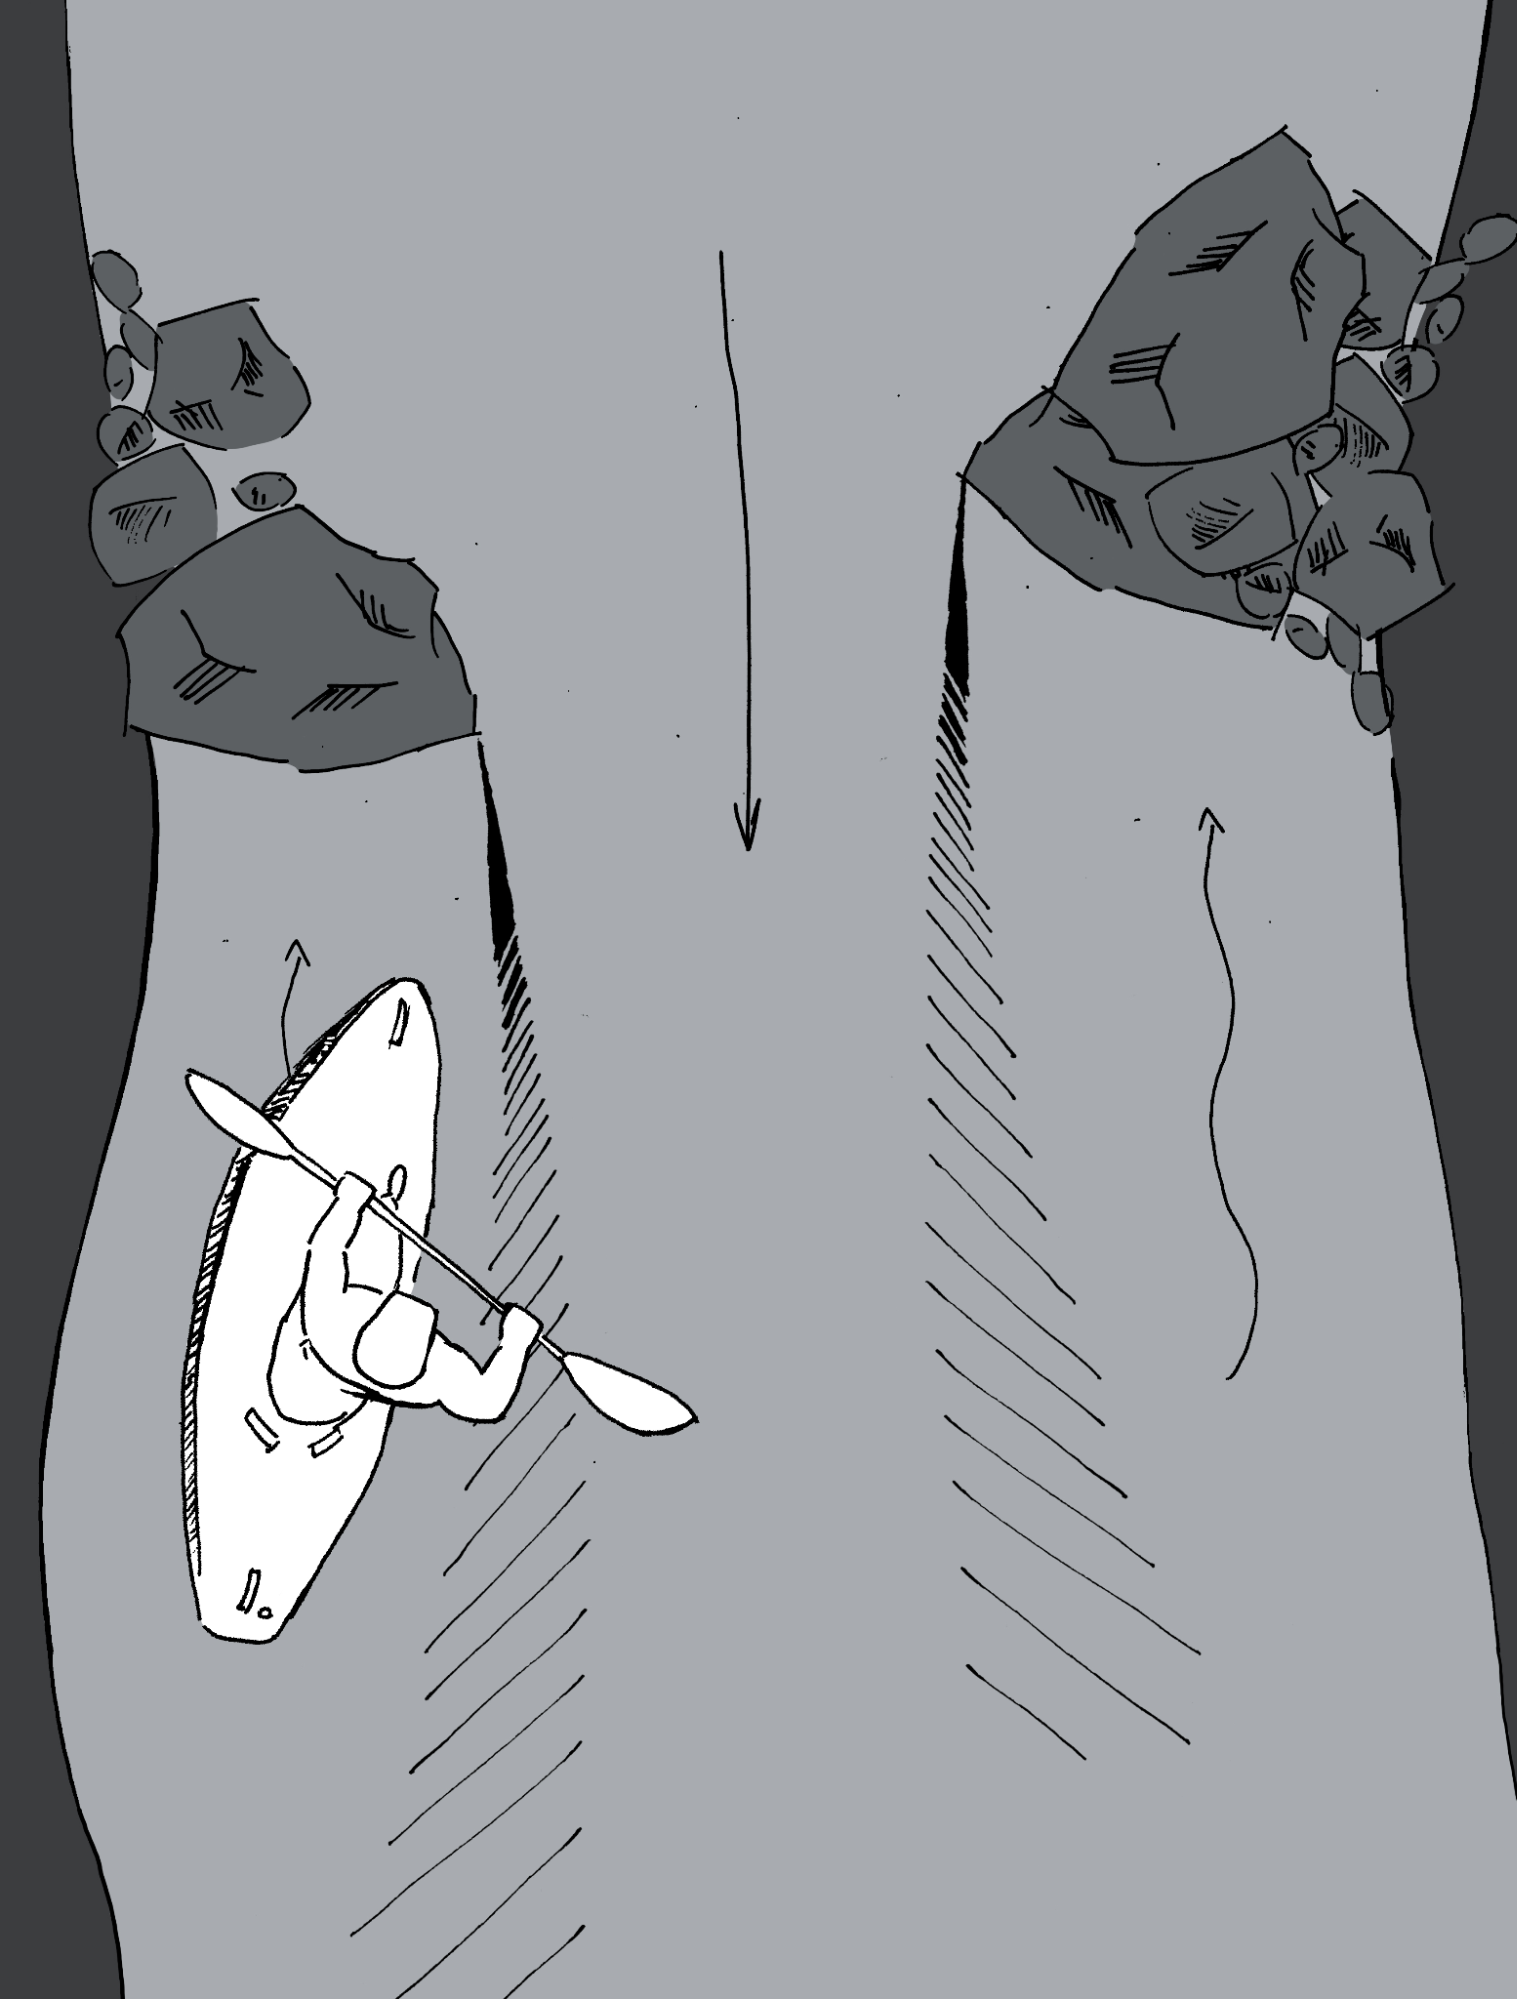
\includegraphics[width=300px]{images/wyjscie_na_nurt.png}
    \caption{Schemat wychodzenia na nurt}
\end{figure}

\end{description}

% ============================================================
%  Rozdział 5 — Manewry
% ============================================================
\section{Manewry}

\begin{tipbox}
\noindent
\begin{minipage}[c]{0.72\linewidth}
  W PrzeWrotce, podobnie jak w kilku innych akademickich klubach kajakowych, praktykuje się tradycję kreślenia palcem znaku wiru na kasku po zanurzeniu ręki w wodzie, jako symboliczne życzenie bezpiecznego spłynięcia.
\end{minipage}
\hfill
\begin{minipage}[c]{0.18\linewidth}
  \centering
  
\includegraphics[width=\linewidth]{images/wir.png}
\end{minipage}
\end{tipbox}

% ------------------------------------------------------------
\subsection{Rozgrzewka}
% ------------------------------------------------------------

Dobrze przeprowadzona rozgrzewka w kajakarstwie górskim realnie zmniejsza ryzyko kontuzji
i poprawia kontrolę łódki. Rozgrzewka ma na celu:

\begin{itemize}[leftmargin=1.5em, itemsep=2pt]
  \item podniesienie temperatury ciała,
  \item przygotowanie stawów i mięśni do pracy w wodzie,
  \item aktywację mięśni stabilizujących,
  \item poprawę koordynacji i czucia ciała,
  \item zmniejszenie ryzyka urazów barków, kręgosłupa i nadgarstków,
  \item mobilizację bioder.
\end{itemize}

\begin{tipbox}
  Czas trwania: 10--15 minut, dopasowany indywidualnie.
  Rozgrzewkę wykonujemy \textbf{na lądzie}, przed wejściem do kajaka.
\end{tipbox}


% ------------------------------------------------------------
\subsection{Przechył}
% ------------------------------------------------------------

Przechył kajaka to kontrolowane przechylenie łodzi na bok (na burtę), wykonywane świadomie przez kajakarza za pomocą pracy bioder i odpowiedniego ułożenia ciała. Bezpośrednio wpływa
na stabilność i sterowność — kajak znacznie lepiej reaguje na ruchy wykonywane w lekkim przechyle, a sztywna, napięta postawa utrudnia panowanie nad łodzią.

Przechył polega na \textbf{uniesieniu jednej burty kajaka i dociążeniu drugiej} poprzez pracę bioder i uniesienie jednego kolana, przy jednoczesnym zachowaniu względnie pionowej pozycji tułowia. Ruch powinien wynikać z kontrolowanego „rolowania" bioder, nie z pochylania całego ciała na bok. Głowa powinna pozostawać możliwie blisko osi kajaka — jej wychylenie na stronę przechyłu znacząco zwiększa ryzyko wywrotki.

Wystarczy \textbf{niewielki, kilkustopniowy przechył}, aby kajak zaczął lepiej skręcać i stabilniej zachowywał się na falach. Zbyt duży przechył bez wsparcia wiosłem może
prowadzić do wywrotki.

Wiosło pełni ważną rolę w utrzymaniu równowagi podczas przechyłu — lekkie podparcie o taflę wody pozwala poczuć stabilność kajaka i zmniejsza strach przed przechyleniem.
Z czasem kajakarz uczy się łączyć pracę bioder, tułowia i wiosła w jeden płynny ruch.

% ------------------------------------------------------------
\subsection{Wsiadanie i wysiadanie z kajaka}
% ------------------------------------------------------------

\textbf{Wsiadanie} najlepiej wykonywać na płytkiej wodzie lub z niskiego, stabilnego brzegu. Kajak ustawiamy równolegle do brzegu lub lekko dziobem pod prąd. Wiosło kładzie się
poprzecznie za kokpitem, opierając jedno pióro o brzeg lub dno, a drugie o kajak — tworzy to stabilny punkt podparcia. Następnie:

\begin{enumerate}[leftmargin=1.5em, itemsep=2pt]
  \item Uchwyć jedną ręką krawędź kokpitu, drugą wiosło.
  \item Usiądź najpierw na tylnej części kokpitu.
  \item Wsuwaj nogi do środka kajaka.
  \item Przenoś ciężar ciała płynnie, utrzymując środek ciężkości nisko.
  \item Ustaw stopy na podnóżkach i sprawdź pozycję przed odbiciem od brzegu.
\end{enumerate}

\textbf{Wysiadanie} wykonuje się w zasadzie w odwrotnej kolejności. Po zatrzymaniu kajaka w spokojnym miejscu lub przy brzegu: stabilizuj łódź wiosłem, wysuń nogi z kokpitu, oprzyj je o dno lub brzeg, powoli przenieś ciężar ciała na zewnątrz. Nie wstawaj gwałtownie — najpierw „usiądź na brzegu" kajaka, a dopiero potem wstań.

\begin{tipbox}
  Zarówno przy wsiadaniu, jak i wysiadaniu najważniejsze są spokój i precyzja ruchów. Pośpiech niemal zawsze kończy się wywrotką. Na rzece wybieraj miejsca w cofce lub osłonięte od prądu.
\end{tipbox}

% ------------------------------------------------------------
\subsection{Wiosłowanie}
% ------------------------------------------------------------

\begin{longtable}{>{\bfseries}p{4.2cm} p{4.9cm} p{4.9cm}}
  \toprule
  \textbf{Cecha} & \textbf{Wiosłowanie szerokie} & \textbf{Wiosłowanie pionowe} \\
  \midrule
  \endfirsthead
  \toprule
  \textbf{Cecha} & \textbf{Wiosłowanie szerokie} & \textbf{Wiosłowanie pionowe} \\
  \midrule
  \endhead
  \bottomrule
  \endfoot

  Cel główny
    & Skręcanie kajaka, manewrowanie
    & Przemieszczanie się do przodu, przyspieszanie \\

  Pozycja wiosła
    & Pióro daleko od kajaka, ruch półkolisty
    & Pióro bliżej kajaka, prowadzone wzdłuż kadłuba \\

  Początek ruchu
    & Przy stopach
    & Przy stopach \\

  Koniec ruchu
    & Przy rufie
    & Przy biodrach \\

  Ruch tułowia
    & Obrót całego torsu
    & Stabilizacja torsu, bardziej izolowany ruch ramienia \\

  Pozycja nadgarstka
    & Naturalna, mniej krytyczna
    & Nadgarstek przecina pole widzenia; wymaga kontroli \\
\end{longtable}

% ------------------------------------------------------------
\subsection{Podpórka}
% ------------------------------------------------------------

Technika służąca do utrzymania równowagi i zapobiegania wywrotce w sytuacji, gdy kajak traci stabilność. Polega na krótkim, dynamicznym oparciu pióra wiosła o powierzchnię wody
w celu uzyskania dodatkowego podparcia. Podpórka nie jest ruchem siłowym — opiera się na właściwym ułożeniu ciała, pracy bioder i odpowiednim kącie pióra względem wody.

Wykonuje się ją, gdy kajak zaczyna przechylać się na jedną burtę. Wiosło trzymane jest nisko, przed kajakarzem, a pióro ustawia się \textbf{płasko} na powierzchni wody po stronie
przechyłu. Łokcie pozostają blisko tułowia, nadgarstki w neutralnej pozycji — chroni to stawy przed urazami. Kluczowym elementem jest jednoczesna \textbf{praca bioder}, które
prostują kajak, podczas gdy wiosło daje krótkie, stabilne podparcie.

\begin{tipbox}
  Ruch podpórki jest szybki i krótki — nie chodzi o opieranie się ciężarem ciała na wiośle, lecz o chwilowe „dotknięcie" wody i powrót do normalnego prowadzenia kajaka.
\end{tipbox}

% ------------------------------------------------------------
\subsection{Promowanie i trawers}
% ------------------------------------------------------------

Dwa podstawowe manewry pozwalające bezpiecznie poruszać się w poprzek nurtu rzeki. Oba opierają się na odpowiednim ustawieniu kajaka względem prądu.

\textbf{Promowanie} polega na przepłynięciu kajakiem w poprzek rzeki bez znoszenia przez nurt (lub przy kontrolowanym znoszeniu). Kajak ustawiony jest pod odpowiednim kątem do prądu — dziobem lekko pod nurt — dzięki czemu siła wody napierająca na burtę równoważy
znoszenie w dół rzeki.

Kajakarz utrzymuje stały kąt kajaka i wykonuje regularne, spokojne pociągnięcia wiosłem.

\begin{itemize}[leftmargin=1.5em, itemsep=2pt]
  \item \textbf{Zbyt mały kąt} — brak przemieszczania się w bok lub problem z wyjściem z cofki.
  \item \textbf{Zbyt duży kąt} — nurt „zabiera" dziób, kajak obraca się dziobem w dół rzeki i jest znoszony.
\end{itemize}

W obu manewrach ważna jest zasada: \textbf{Patrz gdzie płyniesz} — przemieszczamy się tam, gdzie skierowana jest nasza głowa i wzrok. Jeśli uporczywie wpatrujemy się w wodę /
nurt, najpewniej się przewrócimy.


% ------------------------------------------------------------
\subsection{Wchodzenie z cofki}`
% ------------------------------------------------------------

\begin{figure}[H]
    \centering
    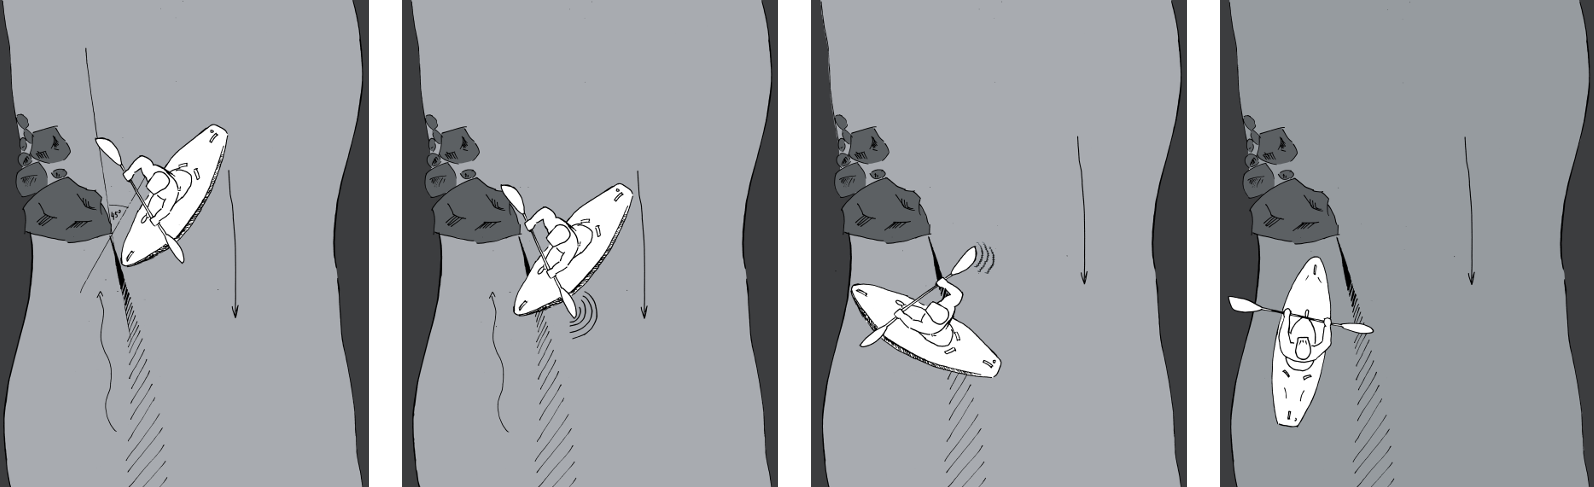
\includegraphics[width=400px]{images/wchodzenie_do_cofki.png}
    \caption{Schemat wejścia do cofki}
\end{figure}

% ------------------------------------------------------------
\subsection{Wychodzenie do cofki}
% ------------------------------------------------------------

\begin{figure}[H]
    \centering
    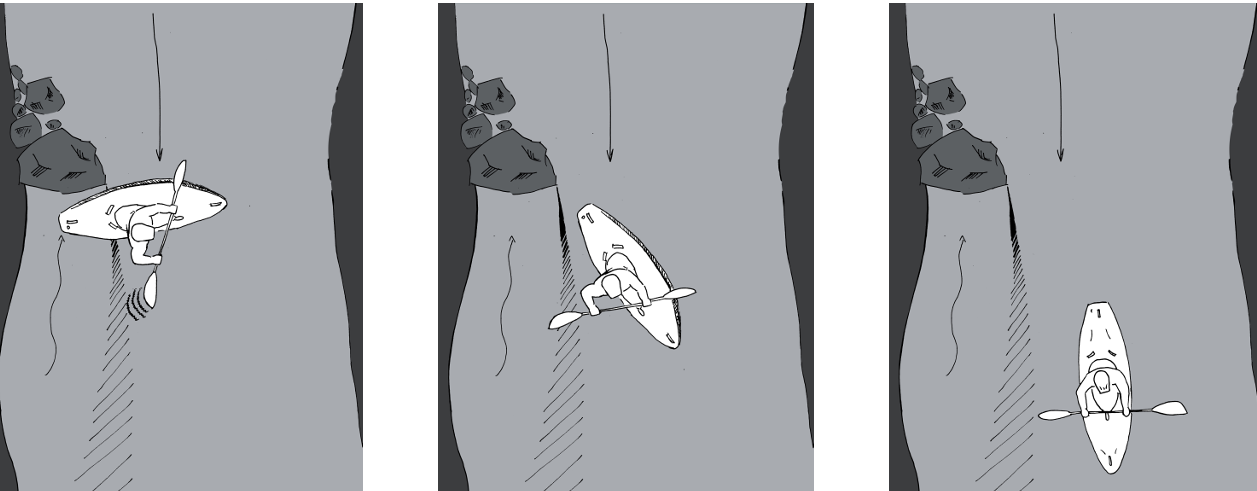
\includegraphics[width=400px]{images/wychodzenie_z_cofki.png}
    \caption{Schemat wyjścia z cofki}
\end{figure}
% ============================================================
%  Rozdział 6 — Bezpieczeństwo
% ============================================================
\section{Bezpieczeństwo}

% ------------------------------------------------------------
\subsection{Znaki wodne}
% ------------------------------------------------------------

\begin{figure}[H]
  \centering
  \begin{subfigure}[t]{0.48\linewidth}
    \centering
    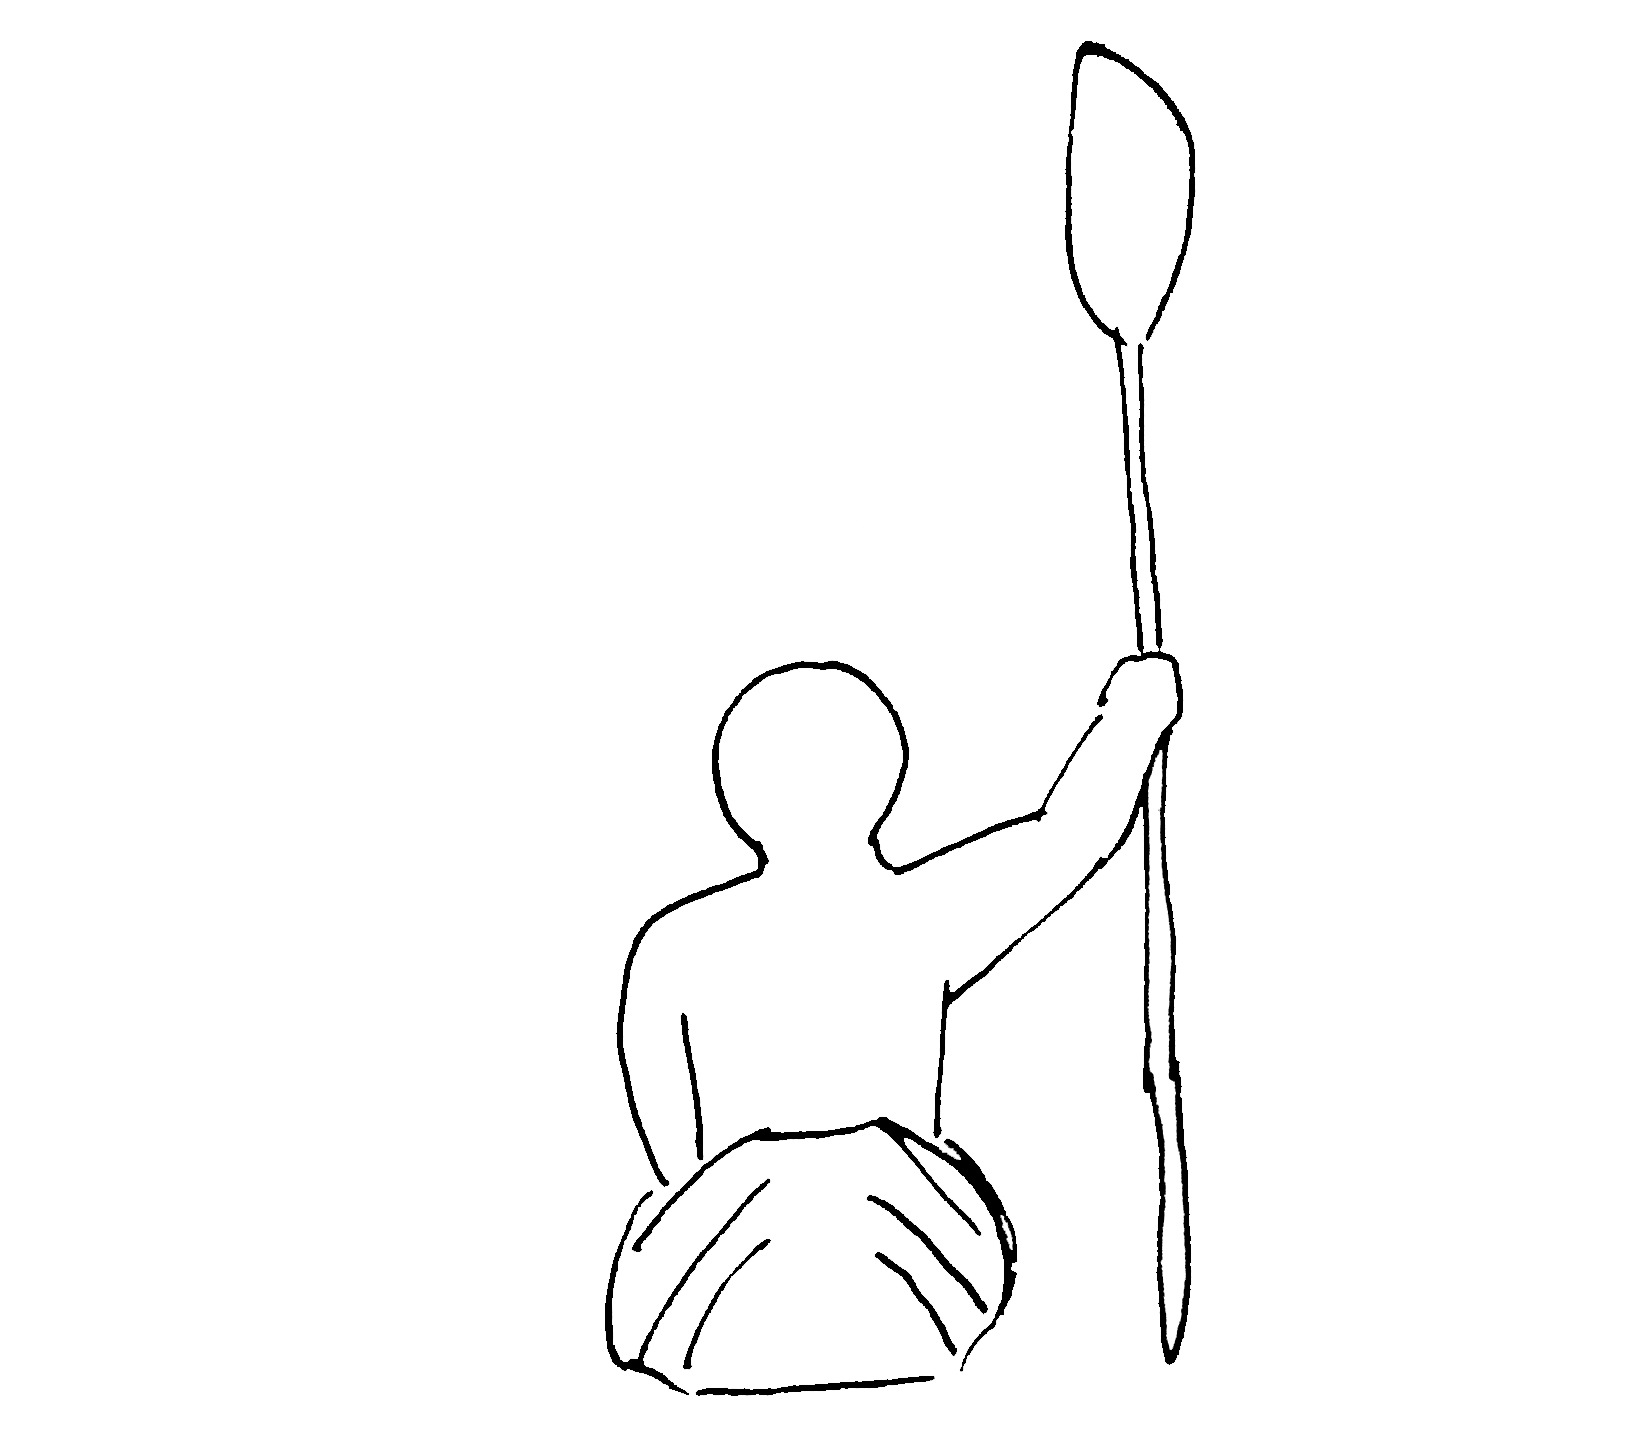
\includegraphics[width=150px]{images/znak_1_plyn.jpg}
    \caption*{Płyń}
  \end{subfigure}
  \hfill
  \begin{subfigure}[t]{0.48\linewidth}
    \centering
    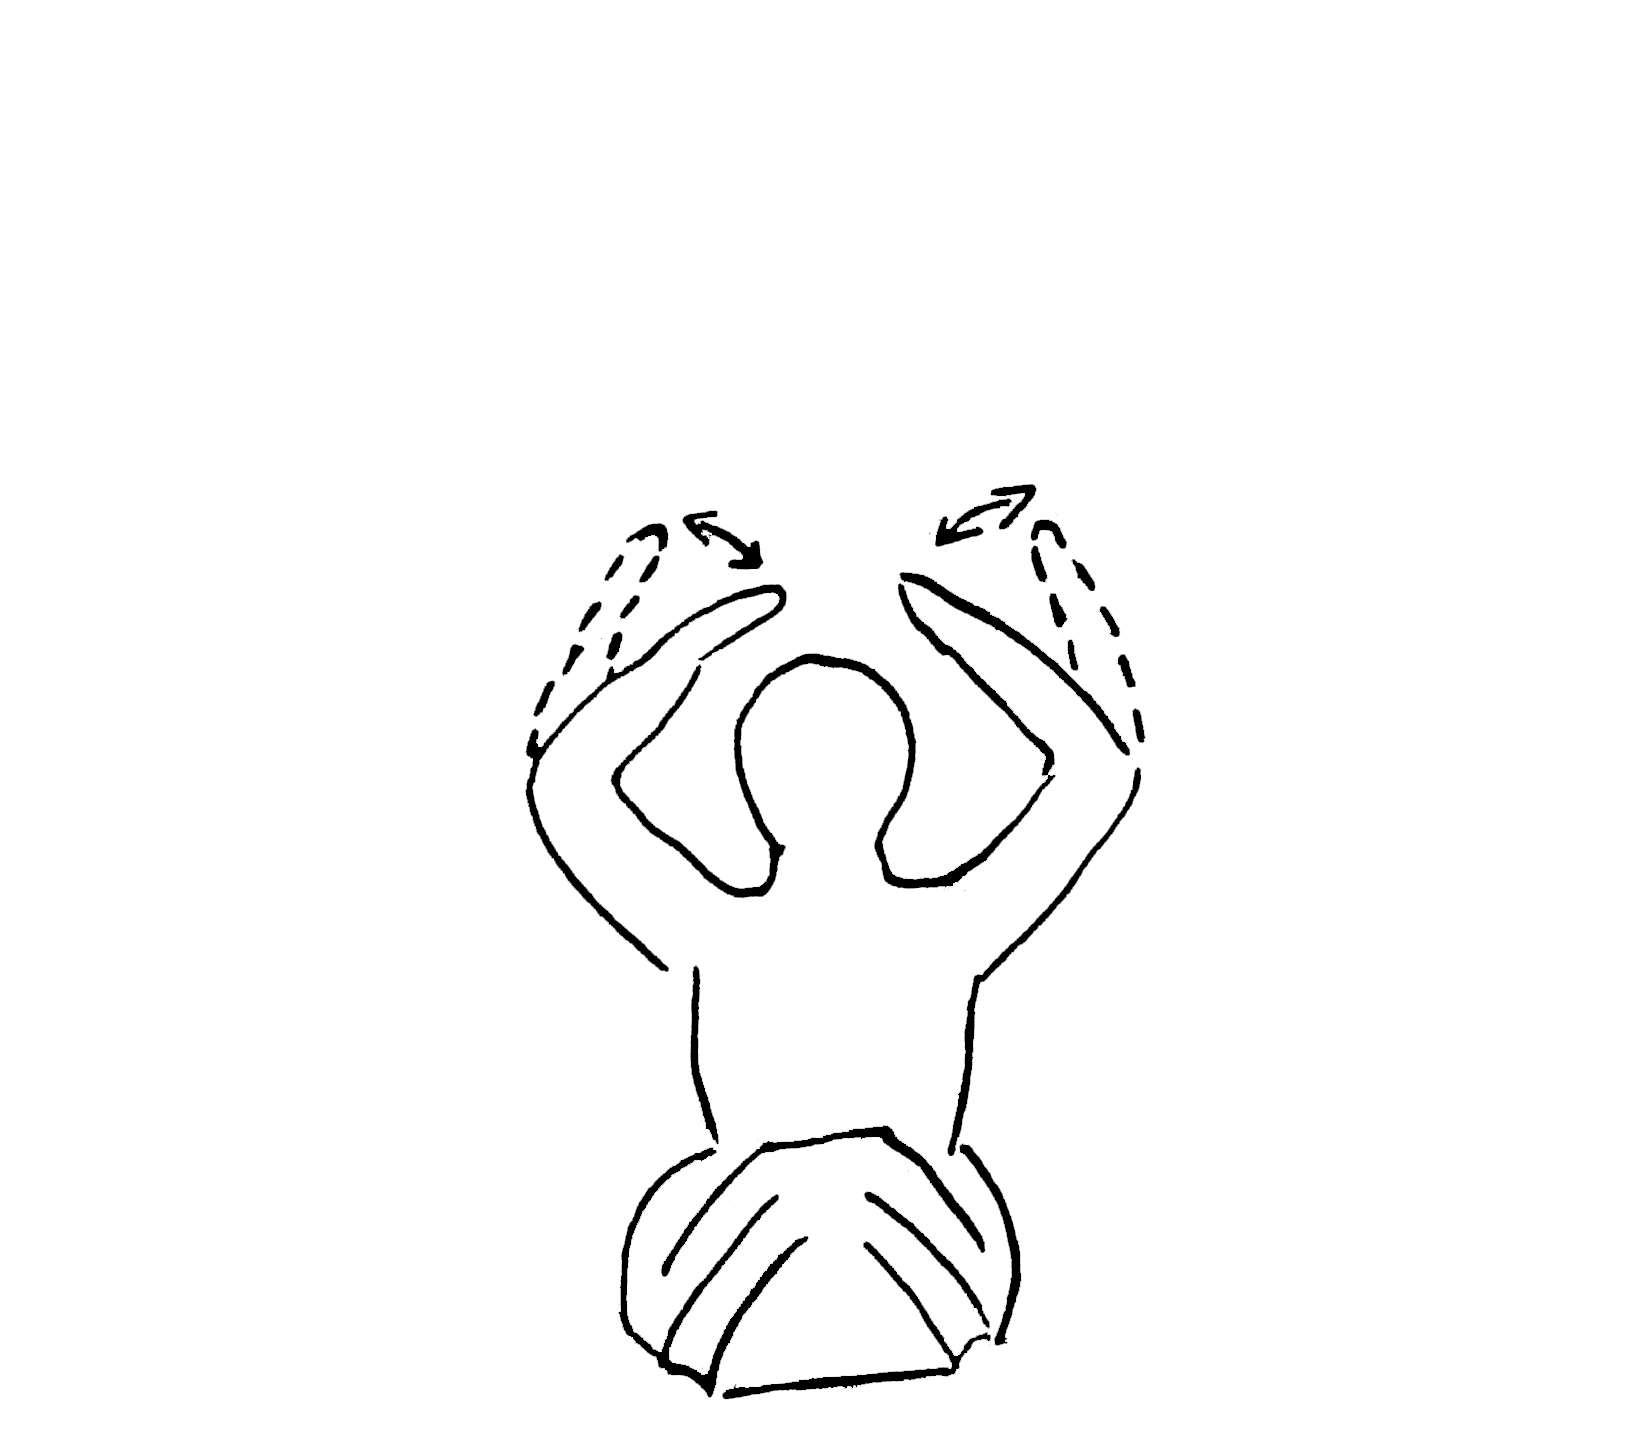
\includegraphics[width=150px]{images/znak_2_do_mnie.jpg}
    \caption*{Do mnie}
  \end{subfigure}
  \begin{subfigure}[t]{0.48\linewidth}
    \centering
    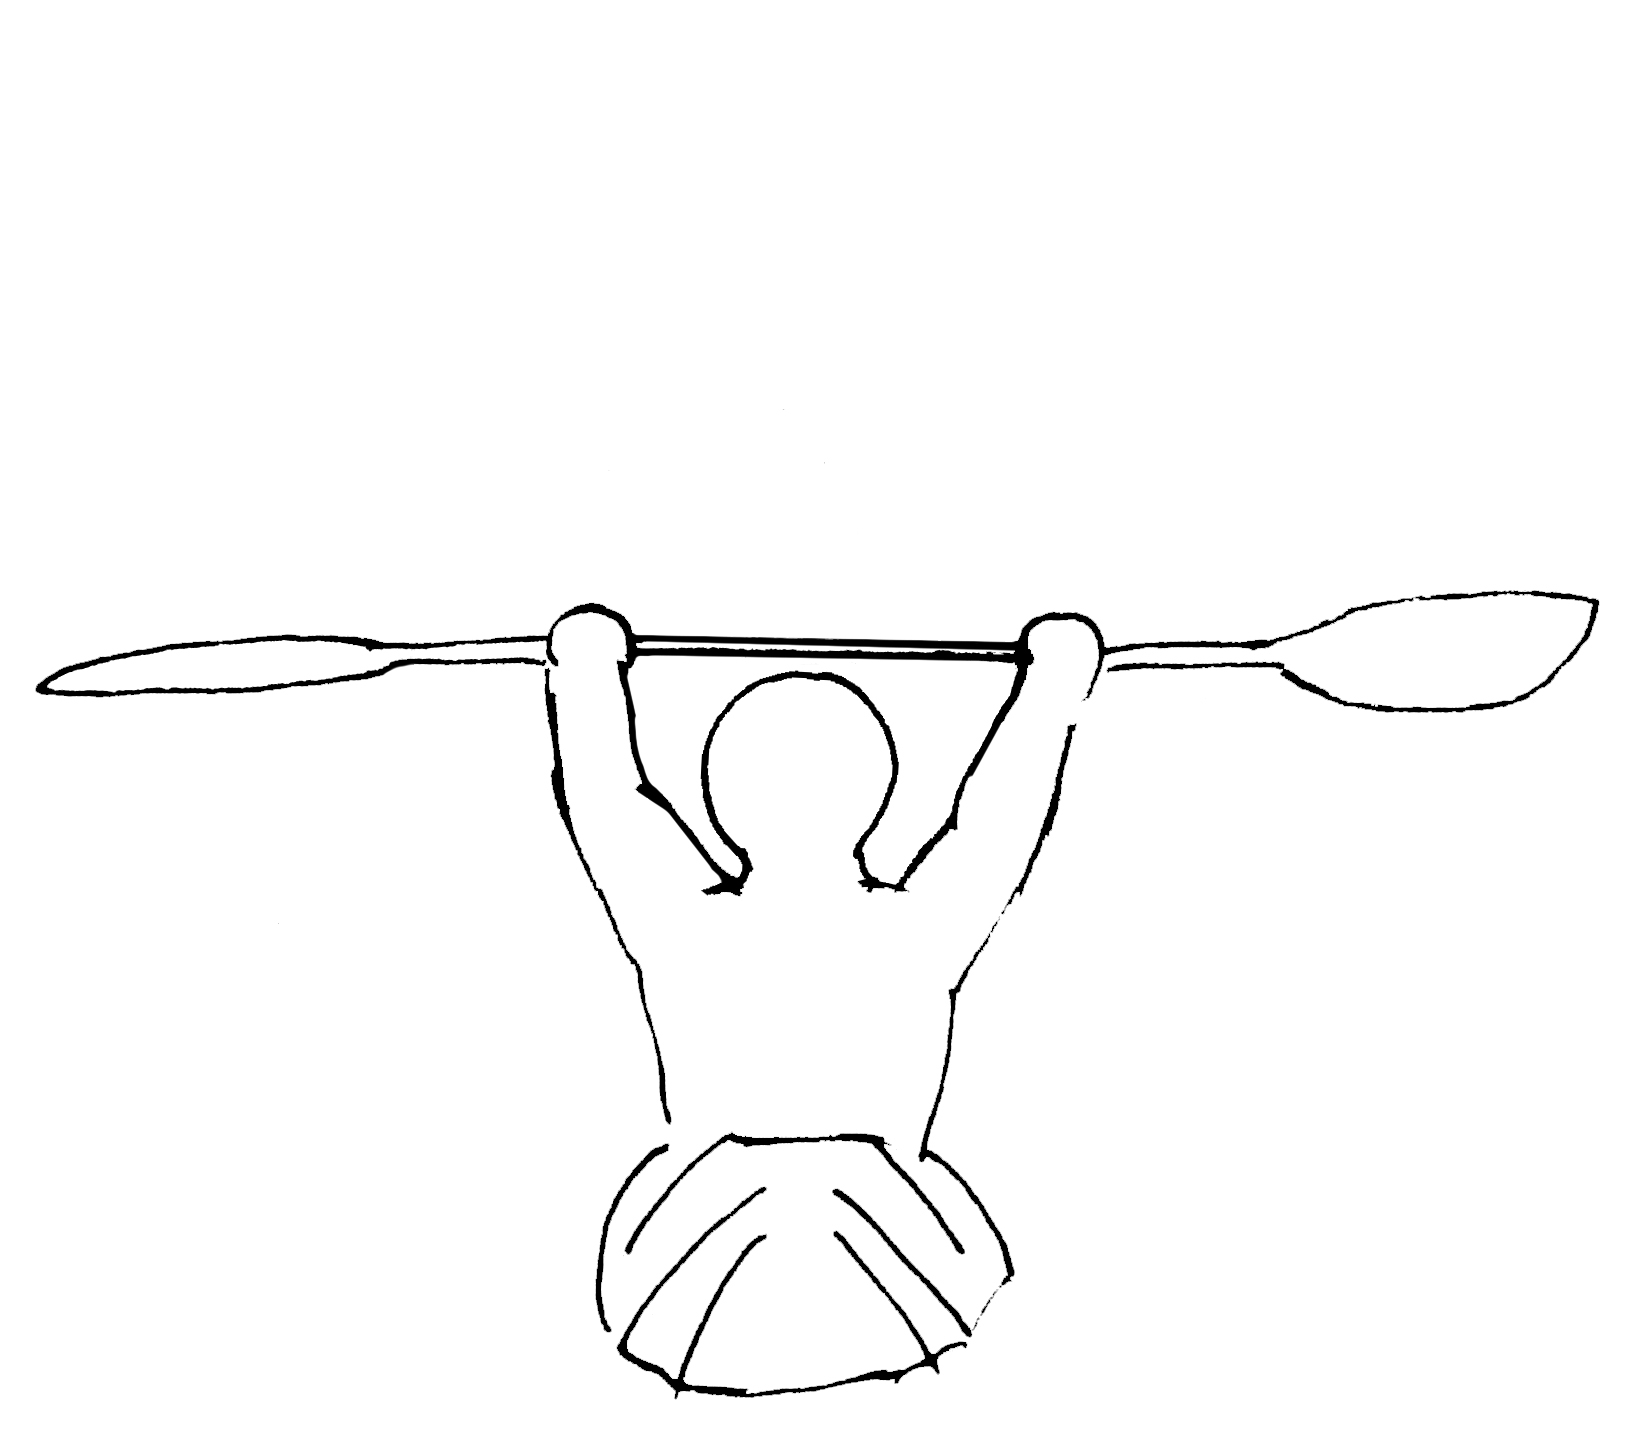
\includegraphics[width=150px]{images/znak_3_stop.jpg}
    \caption*{Stop}
  \end{subfigure}
  \hfill
  \begin{subfigure}[t]{0.48\linewidth}
    \centering
    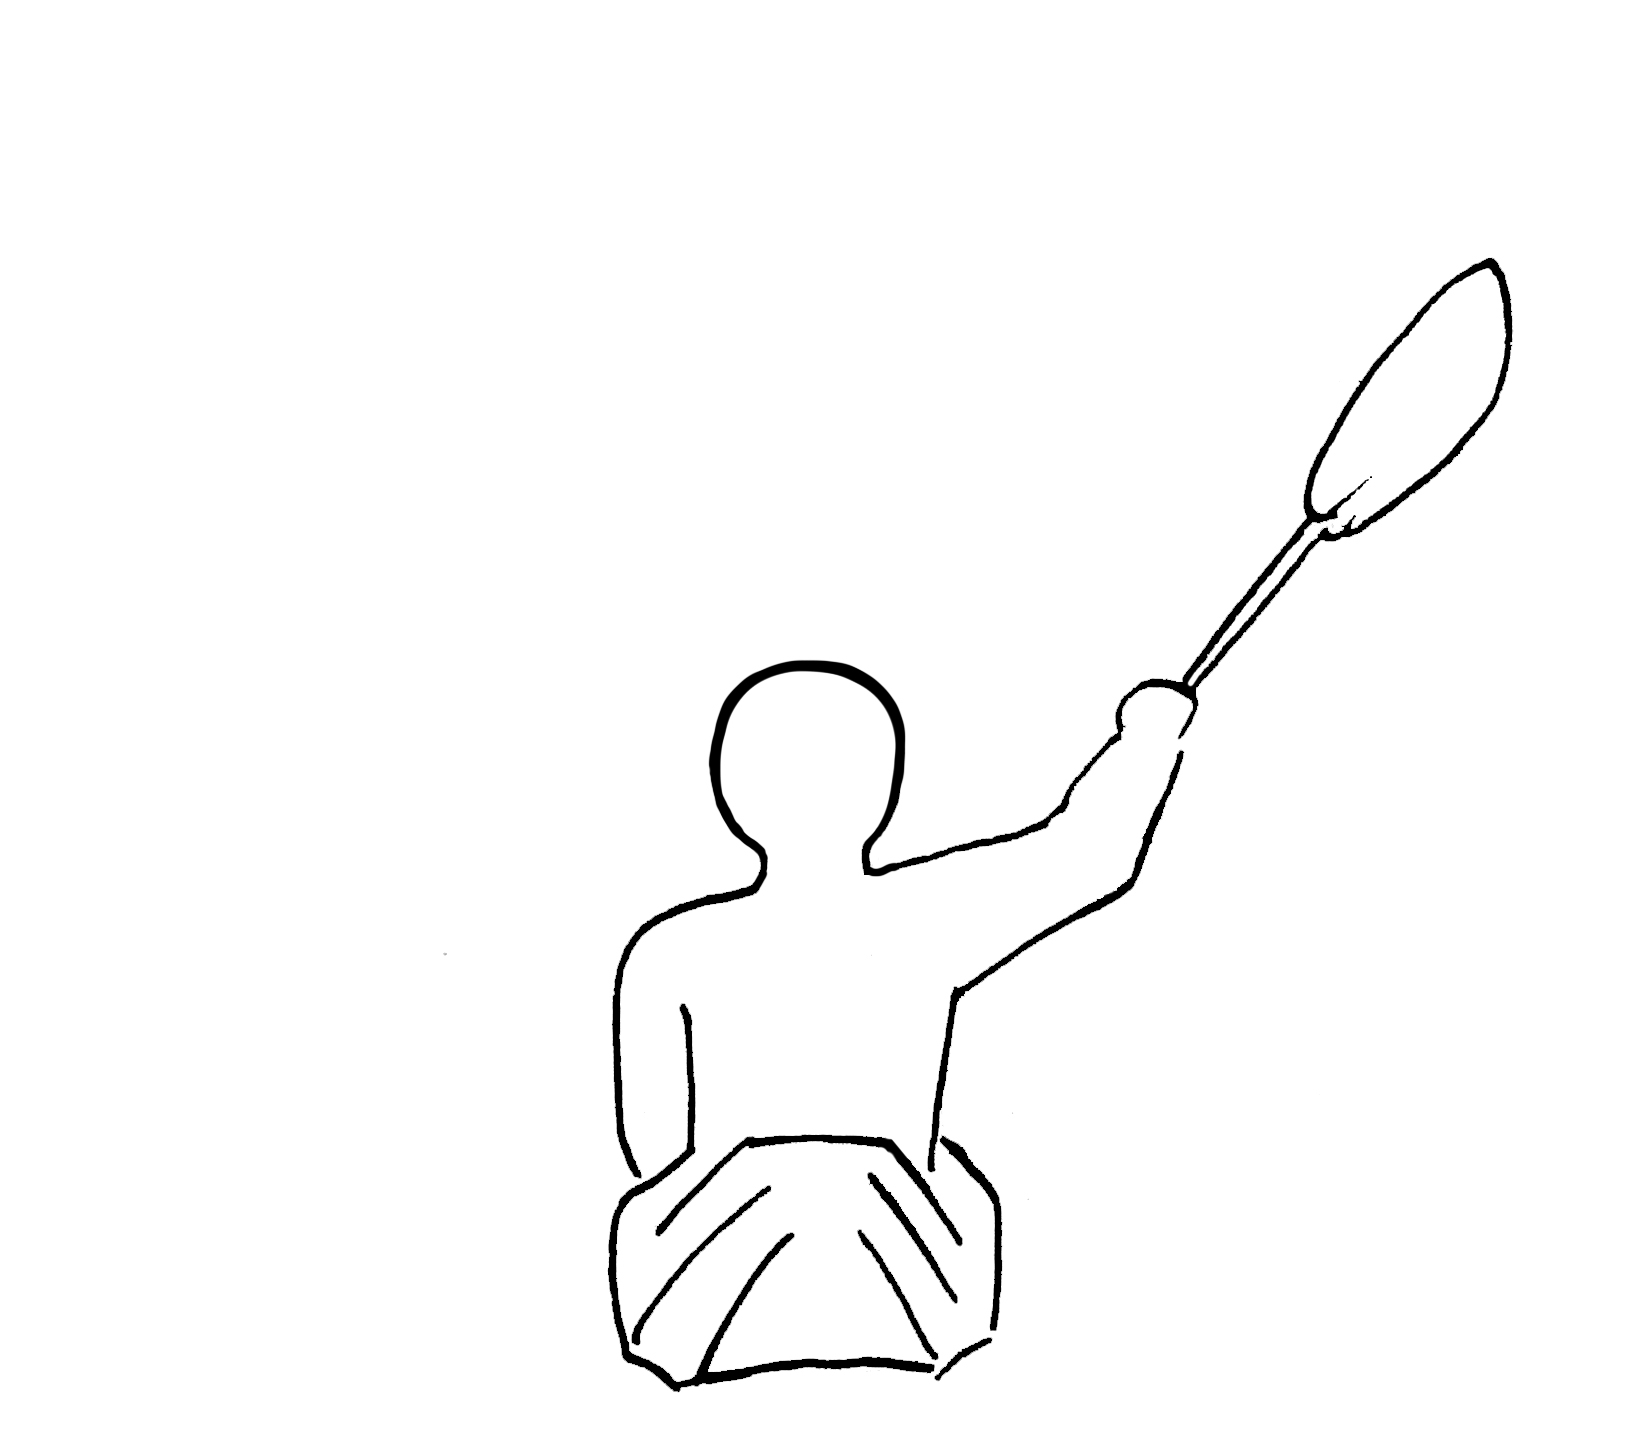
\includegraphics[width=150px]{images/znak_4_plyn_ta_strona.jpg}
    \caption*{Płyń tą stroną}
  \end{subfigure}
  \begin{subfigure}[t]{0.48\linewidth}
    \centering
    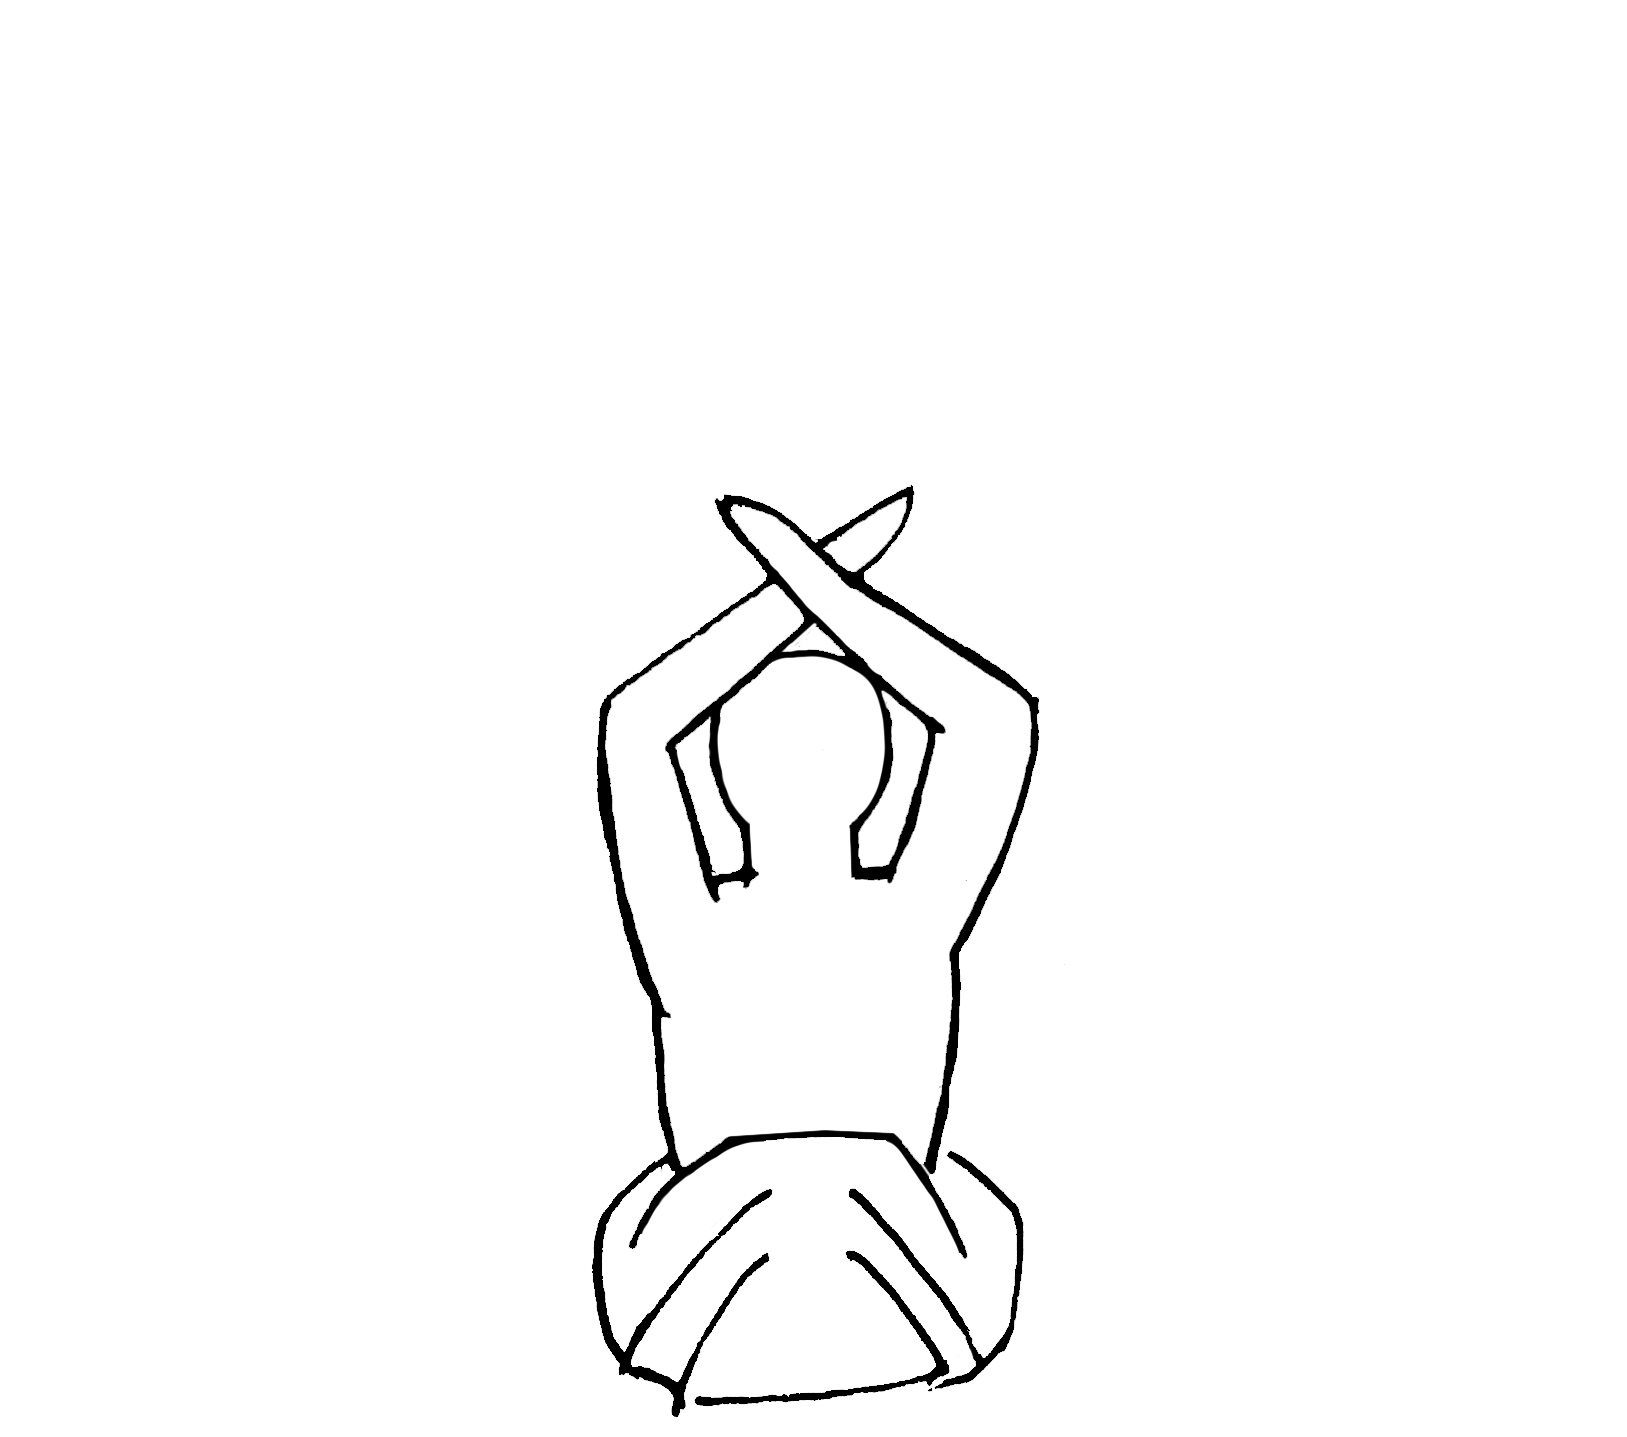
\includegraphics[width=150px]{images/znak_5_koniec.jpg}
    \caption*{Koniec/odcinek niespływalny}
  \end{subfigure}
  \hfill
  \begin{subfigure}[t]{0.48\linewidth}
    \centering
    
\includegraphics[width=50px]{images/znak_6_srodkiem.jpg}
    \caption*{Płyń środkiem}
  \end{subfigure}
  \begin{subfigure}[t]{0.48\linewidth}
    \centering
    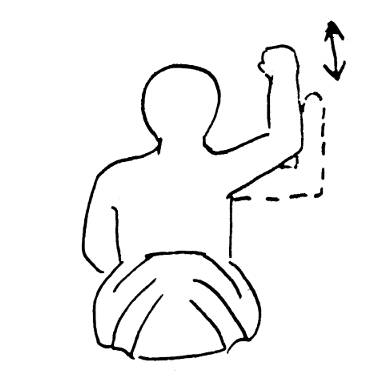
\includegraphics[width=100px]{images/znak_7_przyspiesz.png}
    \caption*{Przyspiesz}
  \end{subfigure}
  \hfill
  \begin{subfigure}[t]{0.48\linewidth}
    \centering
    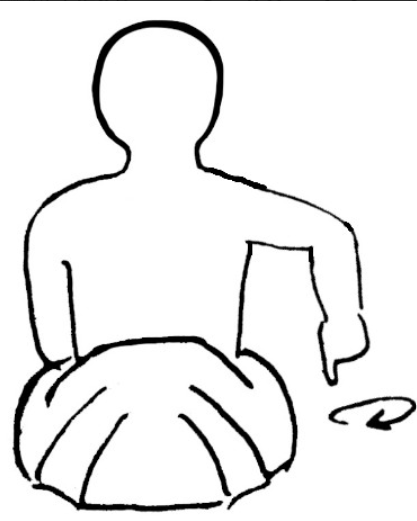
\includegraphics[width=75px]{images/znak_8_cofka.png}
    \caption*{Złap cofkę}
  \end{subfigure}
\end{figure}

\newpage

\begin{figure}[H]
  \ContinuedFloat
  \centering
  \begin{subfigure}[t]{0.48\linewidth}
    \centering
    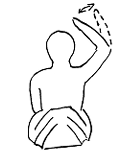
\includegraphics[width=100px]{images/znak_9_ok.png}
    \caption*{Wszystko w porządku}
  \end{subfigure}
  \hfill
  \begin{subfigure}[t]{0.48\linewidth}
    \centering
    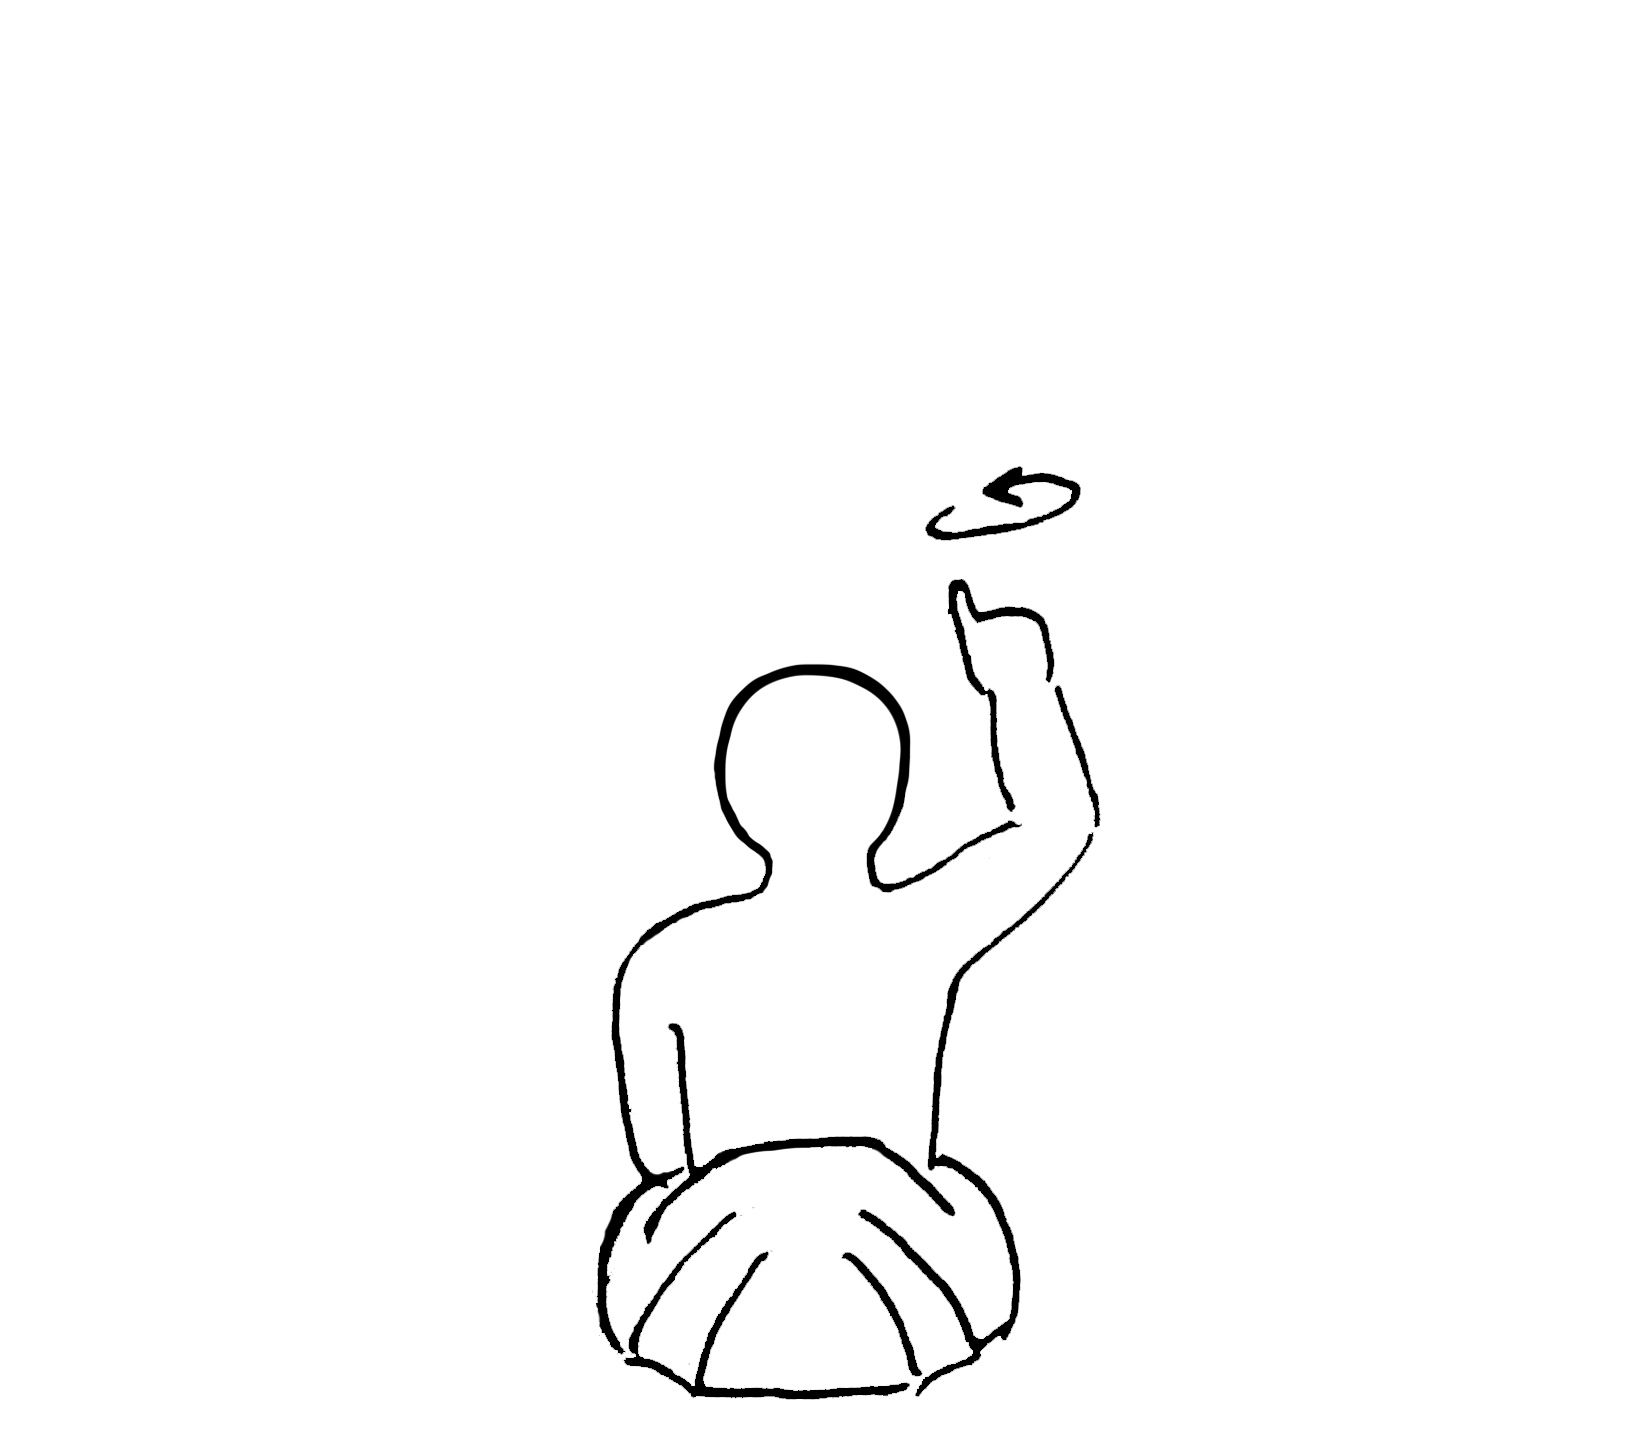
\includegraphics[width=200px]{images/znak_10_kabina.jpg}
    \caption*{Kabina}
  \end{subfigure}
  \begin{subfigure}[t]{0.48\linewidth}
    \centering
    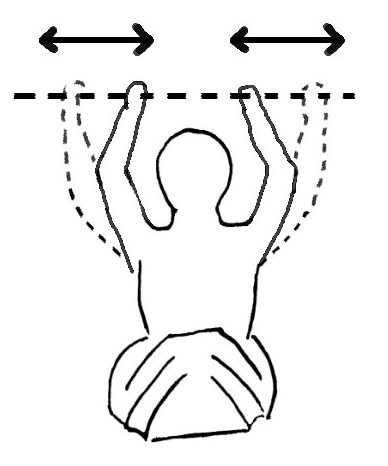
\includegraphics[width=100px]{images/znak_11_wioslo.jpg}
    \caption*{Szukamy wiosła}
  \end{subfigure}
\end{figure}
% ------------------------------------------------------------
\subsection{Komunikacja na wodzie}
% ------------------------------------------------------------

Szum na rzece górskiej nie zawsze pozwala na komunikację werbalną, dlatego przed zejściem na wodę warto ustalić zestaw znaków. Znaki powinny być zawsze przekazane do kolejnej osoby
w szyku i potwierdzone przez każdego członka grupy (jak „głuchy telefon" rękami) — dzięki temu mamy pewność, że dotarły do wszystkich.

Najczęściej używane znaki:

\begin{itemize}[leftmargin=1.5em, itemsep=6pt]
  \item \textbf{Płyń}
  \item \textbf{Stop}
  \item \textbf{Koniec / odcinek niespływalny}
  \item \textbf{Do mnie}
  \item \textbf{Płyń tą stroną}
  \item \textbf{Płyń środkiem}
  \item \textbf{Przyspiesz}
  \item \textbf{Wszystko w porządku}
  \item \textbf{Wiosło}
  \item \textbf{Złap cofkę}
  \item \textbf{Kabina}
\end{itemize}

% ------------------------------------------------------------
\subsection{Filary bezpieczeństwa}
% ------------------------------------------------------------

\subsubsection{Filar 1 — Odpowiednie planowanie}

Dobrze przygotowany spływ pozwala nie tylko uniknąć zagrożeń, ale także zwiększa komfort
uczestników. Proces planowania powinien uwzględniać:

\begin{description}[leftmargin=1.5em, font=\bfseries, style=nextline]

  \item[Dopasowanie poziomu trudności do grupy]
    Należy wziąć pod uwagę wiek, kondycję fizyczną, doświadczenie kajakowe oraz umiejętność
    pływania uczestników.

  \item[Sprzęt dostosowany do umiejętności i trudności spływu]
    Kajaki, wiosła, kamizelki oraz dodatkowe wyposażenie muszą być dostosowane zarówno
    do poziomu zaawansowania uczestników, jak i do charakteru rzeki.

  \item[Zaplanowanie trasy]
    Obejmuje wybór miejsca startu (\emph{put in}) i zakończenia (\emph{take out}), określenie
    długości odcinka i czasu potrzebnego na jego pokonanie. Należy uwzględnić możliwość
    przerw, miejsc biwakowych oraz punktów ewakuacyjnych.

  \item[Warunki atmosferyczne i hydrologiczne]
    Przed wyprawą sprawdź prognozę pogody (opady, temperatura, burze) oraz warunki
    hydrologiczne (poziom wody, prędkość nurtu). Zbyt wysoki lub gwałtownie zmieniający się
    stan rzeki może znacząco zwiększyć stopień trudności spływu.

  \item[Plan awaryjny — plan B, C, a nawet D i E]
    Każdy spływ powinien mieć przygotowany plan awaryjny: skrócenie trasy, zmianę miejsca
    zakończenia lub przerwanie spływu. Elastyczność i gotowość do zmiany pierwotnych założeń
    są niezbędne dla bezpieczeństwa całej grupy.

\end{description}

% ............................................................
\subsubsection{Filar 2 — Wzajemna asekuracja}

\begin{warnbox}
  Kajakarstwo to \textbf{nie} jest sport indywidualny!
\end{warnbox}

Zasady do zapamiętania:

\begin{itemize}[leftmargin=1.5em, itemsep=2pt]
  \item Pomagamy sobie nawzajem.
  \item Trzymamy się grupy.
  \item Słuchamy kierownika.
  \item \textbf{Klepiemy o dzioba!!!}
  \item Obstawiamy miejsca.
  \item Łowimy kabiny.
  \item Podajemy dzióbki.
  \item Ogarniamy się po kabinie.
\end{itemize}

\paragraph{Dzióbek}

Manewr ratowniczy polegający na wykorzystaniu dziobu kajaka partnera w celu wynurzenia się przewróconego kajakarza. Jest to jedna z podstawowych technik asekuracji zespołowej,
szczególnie przydatna dla osób, które nie opanowały jeszcze eskimoski.

Manewr rozpoczyna się w momencie wywrotki. Zamiast podejmować próbę kabinowania się, kajakarz wyciąga dłonie po obu stronach wywróconego kajaka i mocno uderza w burty —
alarmuje tym kajakarzy w okolicy. Partner podpływa do burty prostopadle. Ratowany chwyta dziób kajaka partnera, który stanowi stabilny punkt podparcia umożliwiający wynurzenie się.

\begin{figure}[H]
    \centering
    
\includegraphics[width=400px]{images/dzióbek.jpg}
    \caption{Wizualizacja zachowania kajakarza wołającego o dzióbek}
\end{figure}

\paragraph{Kabina}

Kabinowanie to manewr pozwalający na szybką i bezpieczną ewakuację z kajaka po wywrotce.
Celem jest wydostanie się z kokpitu bez paniki.

\begin{enumerate}[leftmargin=1.5em, itemsep=2pt]
  \item Zachowaj spokój. Pochyl się do przodu — twarz jak najbliżej fartucha
    (\emph{zasada „kryj ryj"}).
  \item Chwyć ucho fartucha i mocno pociągnij do góry i do siebie.
  \item Wykonaj kontrolowane podciągnięcie nóg w kierunku kokpitu.
  \item Przesuń biodra i tułów w stronę otwarcia kokpitu, wykonując coś w rodzaju
    przewrotu w przód ku powierzchni wody.
\end{enumerate}

\textbf{Co po kabinie?}

Jeśli to możliwe, staraj się utrzymać wiosło — może być pomocne w płynięciu wpław.
Po wynurzeniu bezwzględnie staraj się znaleźć na brzegu lub innym bezpiecznym miejscu
poza nurtem. Jeśli jesteś w bardzo silnym nurcie, przyjmij \textbf{pozycję bezpieczną}:
twarz skierowana w dół rzeki, stopy uniesione i skierowane w dół rzeki.

\begin{figure}[H]
    \centering
    
\includegraphics[width=400px]{images/pozycja_bezpieczna.png}
    \caption{Wizualizacja płynięcia w pozycji bezpiecznej}
\end{figure}

\begin{warnbox}
  W nurcie bezwzględnie zakazane jest chodzenie po dnie — istnieje ryzyko zaklinowania
  stopy i utknięcia głową pod wodą.
\end{warnbox}

Pozostali kajakarze często podejmują pływaka na dziób lub rufę:

\begin{itemize}[leftmargin=1.5em, itemsep=3pt]
  \item \textbf{Podjęcie na dziób (Koala)} — chwytamy dziób ratującego; głowa z boku
    dziobu, nigdy przed nim. Jeśli mamy siłę, pomagamy ratującemu przebierając nogami.
  \item \textbf{Podjęcie na rufę} — chwytamy uchwyt na rufie jedno- lub oburącz,
    przyjmując pozycję „supermana".
\end{itemize}

\begin{figure}[H]
    \centering
    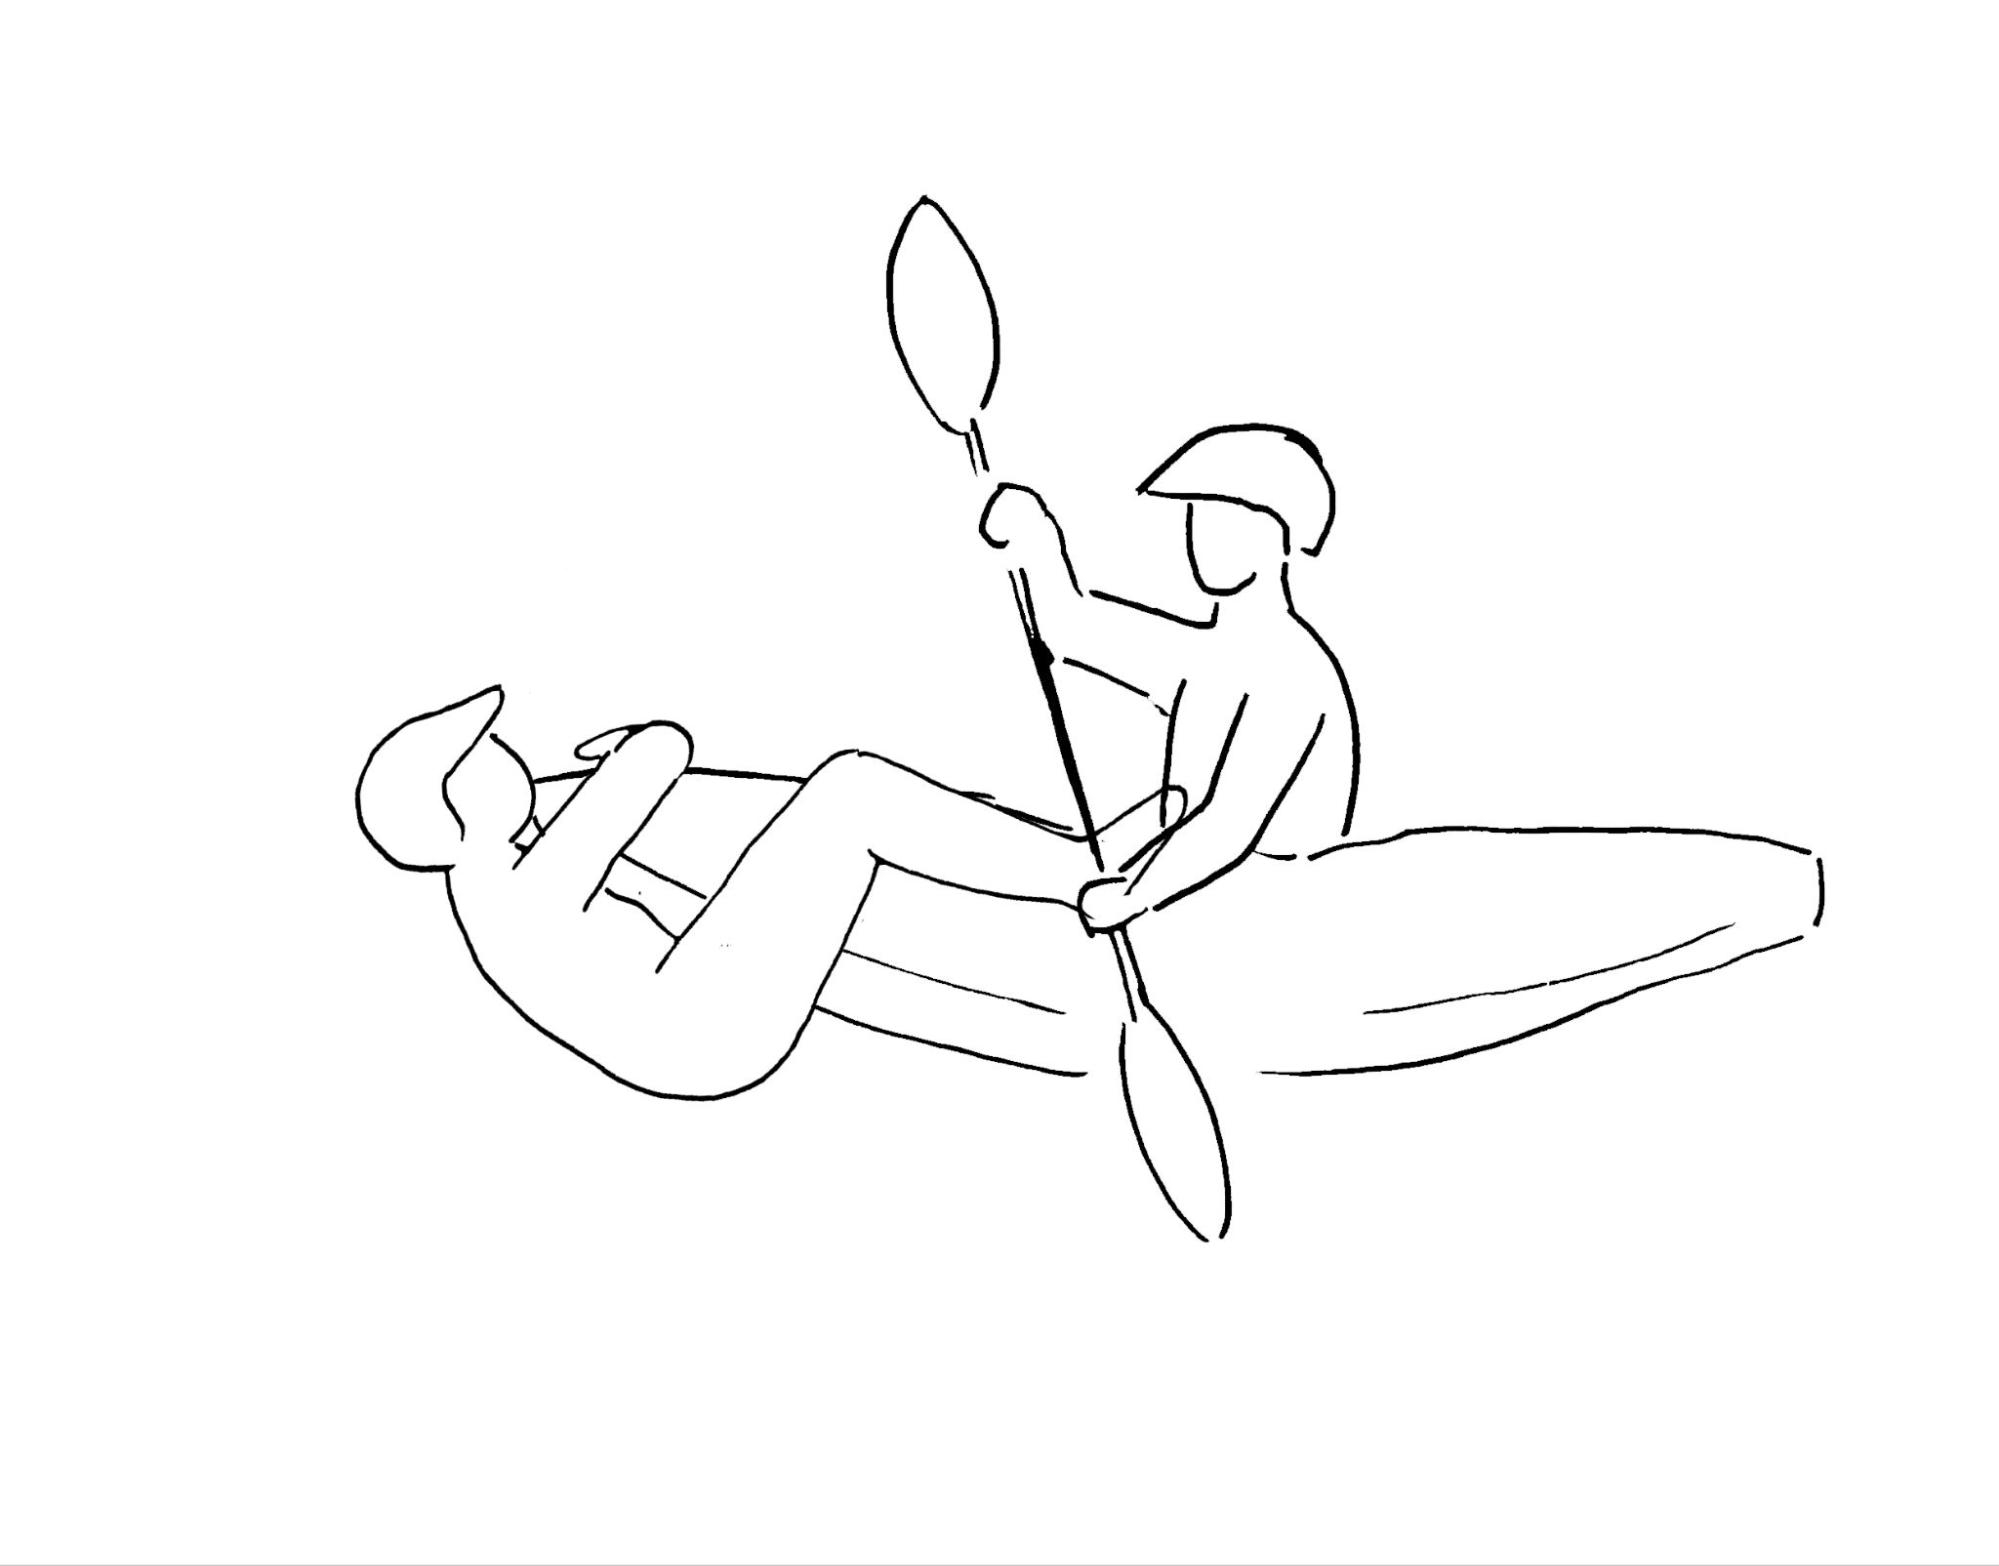
\includegraphics[width=300px]{images/koala.jpg}
    \caption{Wizualizacja manewru holowania na dziobie - koala}
\end{figure}

\begin{tipbox}
  Bezwzględnie stosujemy się do poleceń ratującego. Nigdy nie łapiemy za \textbf{burtę} ratującego — możemy w ten sposób wywrócić naszego ratownika.
\end{tipbox}

\paragraph{Eskimoska}

Eskimoska (rolka) to manewr pozwalający kajakarzowi odwrócić się do pozycji pionowej
po wywrotce bez wychodzenia z kajaka. Opiera się na połączeniu pracy bioder, tułowia
i wiosła.

Ruch powinien być zapoczątkowany z biodra — wykorzystując opór wody na piórze wiosła,
wynurzamy tułów, kontrolując aby \textbf{głowa wynurzyła się na samym końcu}. Kluczowe jest
właściwe wstępne ustawienie wiosła względem kajaka.

\paragraph{Ręka boga}

Manewr ratowniczy używany gdy kajakarz jest przewrócony do góry dnem i nie może sam powrócić
do pionu. Kajakarz asekurujący podpływa obok przewróconego kajaka, sięga ręką i łapie za
rant kokpitu od strony dalszej od siebie. Następnie, naciskając jedną ręką na bliższy bok
i pociągając drugą za dalszy rant, obraca kajak do pozycji pionowej.

Ratowany zawsze utrzymuje pozycję pochyloną do przodu z twarzą jak najbliżej fartucha —
pomaga to ratującemu w wykonaniu manewru.

\paragraph{Asekuracja z brzegu}

Polega na zabezpieczeniu kajakarza znajdującego się w nurcie lub po wywrotce. Osoba
asekurująca stoi mocno w rozkroku lub za kotwicą (np. stabilnym kamieniem).

\textbf{Rzucanie rzutką} wymaga precyzji i przewidzenia nurtu. Przy rzucaniu:

\begin{itemize}[leftmargin=1.5em, itemsep=2pt]
  \item Stój stabilnie na brzegu, \textbf{nigdy} w nurcie.
  \item Nawiąż kontakt wzrokowy z ratowanym i krzyknij \textbf{„RZUTKA!"}
    przed każdym rzutem.
  \item Celuj \emph{przed} kajakarzem — nie w niego bezpośrednio.
  \item Wypuszczaj rzutkę nad wodą, aby lina nie zahaczała o przeszkody.
\end{itemize}

Ratowany po chwyceniu rzutki powinien obrócić się na plecy i skośnie przełożyć linę przed klatką piersiową, po tej samej stronie głowy co ratownik, aby uniemożliwić jej zaplątanie się wokół szyi.

\begin{figure}[H]
    \centering
    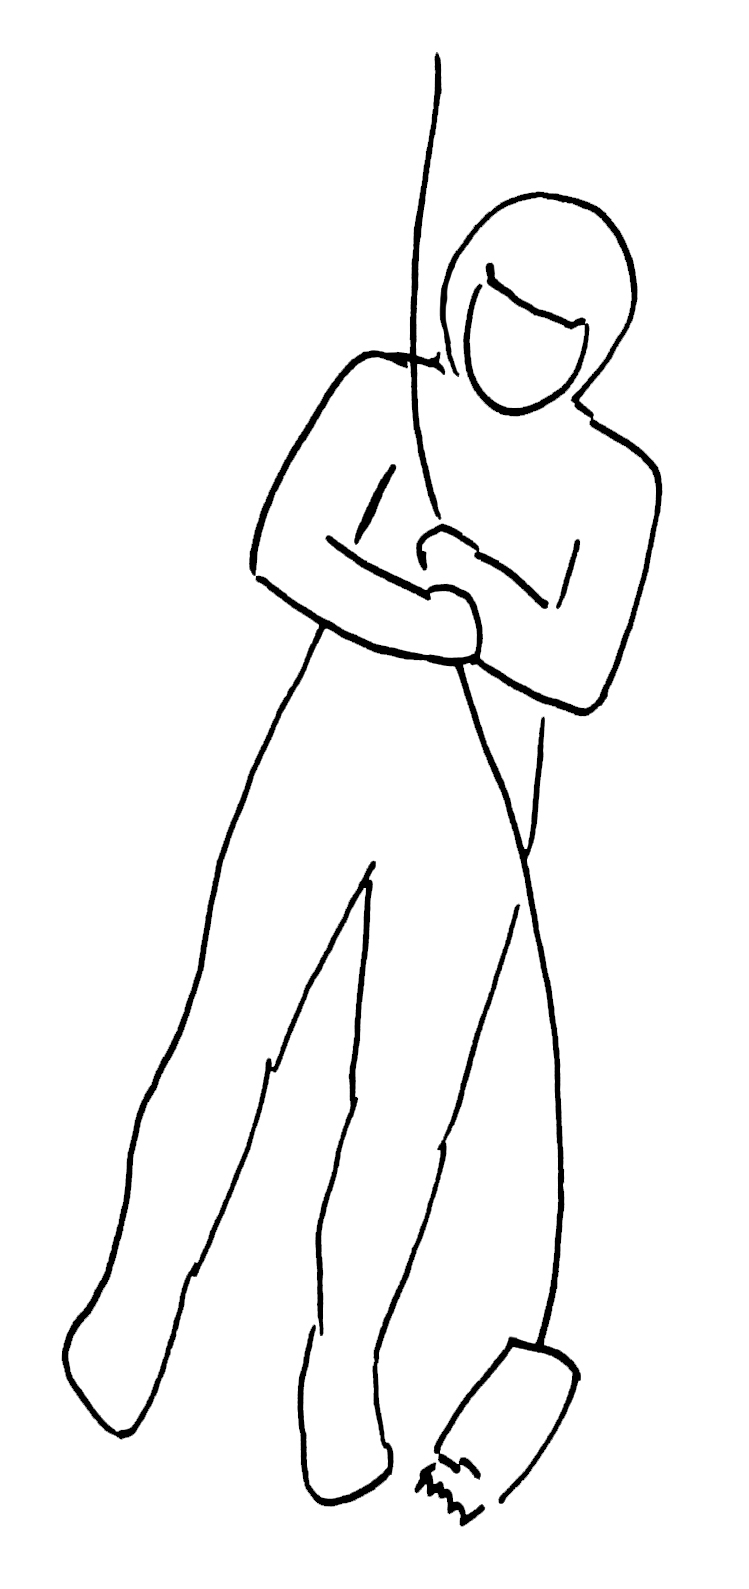
\includegraphics[width=100px]{images/rzutka.jpg}
    \caption{Ułozenie ratowanego po złapaniu rzutki}
\end{figure}

% ............................................................
\subsubsection{Filar 3 — Jednoosobowe kierownictwo}

Jednoosobowe kierownictwo polega na powierzeniu odpowiedzialności za organizację,
bezpieczeństwo i podejmowanie kluczowych decyzji jednej, wyznaczonej osobie —
\textbf{komandorowi spływu}. Na wodzie często dochodzi do sytuacji wymagających
natychmiastowej reakcji; brak jednoznacznego lidera może prowadzić do chaosu.

\begin{warnbox}
  Nigdy nie podważamy decyzji osoby, która rozpoczęła kierownictwo akcją ratunkową.
\end{warnbox}

Cechy komandora spływu:

\begin{description}[leftmargin=1.5em, font=\bfseries, style=nextline]

  \item[Znajomość odcinka rzeki]
    Wiedza o charakterze trasy, miejscach niebezpiecznych, przeszkodach wodnych
    i możliwościach ewakuacji pozwala na odpowiednie przygotowanie i szybkie reagowanie.

  \item[Doświadczenie kajakowe]
    Umożliwia trafną ocenę warunków hydrologicznych i atmosferycznych oraz przewidywanie
    potencjalnych zagrożeń.

  \item[Zdecydowanie]
    Komandor musi potrafić jasno wydawać polecenia i egzekwować ich wykonanie, nawet gdy
    są niepopularne (np. przerwanie spływu lub zmiana trasy).

  \item[Umiejętność działania pod presją]
    Sytuacje awaryjne wiążą się z presją czasu. Komandor powinien zachować spokój, logicznie
    analizować sytuację i podejmować racjonalne decyzje minimalizujące ryzyko dla grupy.

\end{description}

% ------------------------------------------------------------
\subsection{Szyk płynięcia}
% ------------------------------------------------------------

\begin{description}[leftmargin=1.5em, font=\bfseries]
  \item[Zielona Latarnia]
    Pierwsza płynąca osoba (otwierający). Płynie pierwszy, wyznacza linię płynięcia —
    nie wyprzedza się jej.
  \item[Czerwona Latarnia]
    Ostatnia płynąca osoba. Nikt nie pozostaje za nią.
\end{description}

% ------------------------------------------------------------
\subsection{Apteczka}
% ------------------------------------------------------------

\begin{longtable}{>{\bfseries}p{5.5cm} >{\centering}p{1.8cm} p{6.5cm}}
  \toprule
  \textbf{Element} & \textbf{Ilość} & \textbf{Zastosowanie} \\
  \midrule
  \endfirsthead
  \toprule
  \textbf{Element} & \textbf{Ilość} & \textbf{Zastosowanie} \\
  \midrule
  \endhead
  \bottomrule
  \endfoot

  Rękawiczki                       & 3--4 pary  & Ochrona ratownika \\
  Gaza jałowa                      & 5--8 szt.  & Opatrywanie ran \\
  Bandaż elastyczny                & 2 szt.     & Skręcenia, stabilizacja \\
  Bandaż zwykły                    & 2 szt.     & Mocowanie opatrunków \\
  Bandaż elastyczny siatkowy       & 1 szt.     & Mocowanie opatrunków \\
  Plastry z opatrunkiem            & zestaw     & Drobne rany \\
  Plastry ściągające (stripy)      & 1 zestaw   & Zamknięcie ran ciętych \\
  Plaster w rolce (mocny)          & 1 szt.     & Mocowanie, wzmacnianie \\
  Taśma izolacyjna (PVC)*          & 1 rolka    & Usztywnienia, naprawy, opatrunki awaryjne \\
  Chusta trójkątna                 & 1 szt.     & Unieruchomienie kończyn \\
  Koc termiczny (NRC)              & 1--2 szt.  & Ochrona przed hipotermią \\
  Środek do dezynfekcji            & 1 szt.     & Oczyszczanie ran \\
  Opaska uciskowa / staza          & 1 szt.     & Masowe krwotoki \\
  Nożyczki ratownicze              & 1 szt.     & Cięcie ubrań, bandaży \\
  Maska do RKO                     & 1 szt.     & Bezpieczna resuscytacja \\
  Pęseta                           & 1 szt.     & Drzazgi, kleszcze \\
  Folia / etui wodoszczelne        & 1 szt.     & Ochrona apteczki \\
  Instrukcja pierwszej pomocy      & 1 szt.     & Wsparcie w stresie \\
  Lista wyposażenia apteczki       & 1 szt.     & Rewizja i uzupełnienie \\
\end{longtable}
% ============================================================
%  Rozdział 7 — Poszkoleniówkowe PiO
% ============================================================
\section{Poszkoleniówkowe PiO}

Jeśli tutaj dotarłeś/aś, oznacza to, że jesteś pełnoprawnym członkiem klubu i masz takie
same przywileje i obowiązki jak ci długoletni. Regulaminy znajdziesz na naszym Discordzie,
na kanale \texttt{\#przydatne-informacje}.

Wzięcie udziału w szkoleniu gwarantuje opłaconą składkę na najbliższe pół roku.
Co pół roku skarbnik PrzeWrotki przypomina o jej opłaceniu — wynosi ona \textbf{100~zł/semestr}.
Przewidziane są benefity za terminowe płacenie!

% ------------------------------------------------------------
\subsection*{Komunikacja w klubie — Discord}
\addcontentsline{toc}{subsection}{Komunikacja w klubie — Discord}
% ------------------------------------------------------------

Wszystkie wyjazdy klubowe, integracje, pytania i zmiany organizacyjne ogłaszane są
na klubowym Discordzie. Jest on podzielony na kanały — przykładowo, cotygodniowe pływanie
na Odrze jest na \texttt{\#wroclaw-plywanie}, a dalsze wyjazdy w góry — na \texttt{\#whitewater}.

Z początku ilość kanałów może wydawać się przytłaczająca, ale z czasem wszystko stanie się
jasne. Dostęp do Discorda otrzymasz tuż po skończeniu szkoleniówki.

% ------------------------------------------------------------
\subsection*{Godzinki — co to?}
\addcontentsline{toc}{subsection}{Godzinki — co to?}
% ------------------------------------------------------------

Godzinki są naszą walutą klubową. Za godzinki mamy umożliwione wypożyczenie sprzętu
i korzystanie z klubowych atrakcji, a możemy je zarobić uczciwą pracą — przy naprawach
sprzętowych, organizacji spływów, szkoleniu kolejnych pokoleń kajakarzy i wielu innych.

Wszystkie szczegóły i cennik znajdują się w regulaminach na Discordzie.
\textbf{Każdy nowy członek klubu dostaje na swoje konto 6 godzinek.}

% ------------------------------------------------------------
\subsection*{Jak wypożyczyć sprzęt?}
\addcontentsline{toc}{subsection}{Jak wypożyczyć sprzęt?}
% ------------------------------------------------------------

Do zarządzania sprzętem służy nasza autorska aplikacja przeglądarkowa — \textbf{PrzeWrotkApp}:

\begin{center}
  \url{https://app.przewrotka.org/}
\end{center}

Możesz ją dodać do ekranu głównego na swoim telefonie — będzie wtedy działać jak klasyczna
aplikacja. Po skończonej szkoleniówce otrzymasz wiadomość na maila z instrukcjami logowania.

\begin{tipbox}
  Jeśli zauważyłeś (lub spowodowałeś :P) jakiekolwiek wady sprzętu — dodaj je
  w komentarzach i zgłoś to sprzętowcowi, żeby nie nadziać następnej osoby
  na nieprzyjemną niespodziankę!
\end{tipbox}

% ------------------------------------------------------------
\subsection*{Jak zarobić godzinki?}
\addcontentsline{toc}{subsection}{Jak zarobić godzinki?}
% ------------------------------------------------------------

Wiele wydarzeń ogłaszanych na Discordzie wymaga pomocy. Jeśli wykażesz się inicjatywą,
zostaniesz doceniony! Możesz też samodzielnie zorganizować jakieś wydarzenie klubowe
(kajakowe lub nie) — szczegóły w cenniku na \texttt{\#przydatne-informacje}.

Dodatkowo, w zakładce \emph{Zarób} w aplikacji znajdziesz sprzęty z uszkodzeniami
czekające na opiekę.

% ------------------------------------------------------------
\subsection*{Kontakt z zarządem}
\addcontentsline{toc}{subsection}{Kontakt z zarządem}
% ------------------------------------------------------------

\begin{description}[leftmargin=1.5em, font=\bfseries]
  \item[Mateusz (Blue) Soszyński — Prezes]
    Kwestie organizacyjne.
  \item[Kacper (Kacperek) Dąbek — Sprzętowiec]
    Dobór, wypożyczenie i naprawy sprzętu.
  \item[Karolina (Facetka) Sienkiewicz — Szkoleniowiec]
    Dokształcanie się i bycie lepszym kajakarzem.
  \item[Zuzanna Ejsymont — Skarbnik]
    Wszystkie kwestie finansowe.
  \item[Alicja Pernal — Godzinkowa]
    Zgłaszanie wykonanej pracy i rozliczanie godzinek.
  \item[Zuzanna Ejsymont, Zuzanna Kawczyńska, Filip Madzia, Michał Markiewicz (Fantom) — PR]
    Instagram i Facebook. Chętnie przyjmują zdjęcia i opowieści z wypraw.
\end{description}

% ------------------------------------------------------------
\subsection*{Możliwości pływania}
\addcontentsline{toc}{subsection}{Możliwości pływania}
% ------------------------------------------------------------

Bądź na bieżąco z Discordem — każde wydarzenie klubowe ląduje właśnie tam. Poza wyjazdami
ogłaszane są też cykliczne spotkania na stacjonarne ćwiczenie eskimosek na Odrze oraz
spotkania towarzyskie na barce.

Pamiętaj, że Ty też możesz organizować wyjazdy i spotkania — jeśli nie wiesz jak,
rzuć pomysł na Discordzie, chętni się znajdą.

% ------------------------------------------------------------
\subsection*{Gdzie szukać informacji o rzekach?}
\addcontentsline{toc}{subsection}{Gdzie szukać informacji o rzekach?}
% ------------------------------------------------------------

\begin{itemize}[leftmargin=1.5em, itemsep=4pt]
  \item Zapytać bardziej doświadczonych kajakarzy!
  \item Strony internetowe:
    \href{http://wiki.bystrze.pl}{\texttt{wiki.bystrze.pl}},
    \href{http://rivermap.org}{\texttt{rivermap.org}},
    \href{http://wkw.wloclawek.pttk.pl/kajszl.html}{\texttt{wkw.wloclawek.pttk.pl}}
  \item Aplikacje: \emph{Zwałkowe Pegle}, \emph{RiverApp}, \emph{whitewater.guide}
\end{itemize}

% ------------------------------------------------------------
\subsection*{Planowanie spływu jako komandor}
\addcontentsline{toc}{subsection}{Planowanie spływu jako komandor}
% ------------------------------------------------------------

Przydatne narzędzia:

\begin{itemize}[leftmargin=1.5em, itemsep=2pt]
  \item Notatka z zaznaczonymi miejscami charakterystycznymi (mosty, progi, łatwo
    rozpoznawalne punkty)
  \item Pinezki Google Maps
  \item Grupa na Messengerze
  \item Excel z uczestnikami i numerami telefonów
\end{itemize}

% ------------------------------------------------------------
\subsection*{Jak jeszcze mogę wesprzeć klub?}
\addcontentsline{toc}{subsection}{Jak jeszcze mogę wesprzeć klub?}
% ------------------------------------------------------------

Możesz przekazać \textbf{1{,}5\% podatku} na rzecz WKK PrzeWrotka:

\begin{center}
  \begin{tabular}{ll}
    \textbf{KRS:}              & 0000270261 \\
    \textbf{Cel / tytuł:}      & WKK Przerwotka 21794 \\
    \textbf{Numer konta:}      & 35 2030 0045 1110 0000 0382 5640 \\
  \end{tabular}
\end{center}
% ============================================================
%  Rozdział 8 — Regulamin Szkolenia
% ============================================================
\section{Regulamin Szkolenia z Podstaw Kajakarstwa Górskiego 2026}

% ------------------------------------------------------------
\subsection*{§1. Organizator}
\addcontentsline{toc}{subsection}{§1. Organizator}
% ------------------------------------------------------------

Organizatorem szkolenia jest \textbf{Wrocławski Klub Kajakowy „PrzeWrotka"} (dalej:
Organizator).

% ------------------------------------------------------------
\subsection*{§2. Charakter szkolenia}
\addcontentsline{toc}{subsection}{§2. Charakter szkolenia}
% ------------------------------------------------------------

\begin{itemize}[leftmargin=1.5em, itemsep=2pt]
  \item Szkolenie ma charakter sportowy i obejmuje zajęcia teoretyczne oraz praktyczne,
    w tym zajęcia basenowe oraz spływy kajakowe.
  \item Ze względu na intensywność ćwiczeń wymagających dobrej kondycji fizycznej oraz
    stabilnego stanu psychicznego, uczestnicy zobowiązani są do przestrzegania niniejszego
    regulaminu.
\end{itemize}

% ------------------------------------------------------------
\subsection*{§3. Ochrona danych osobowych (RODO)}
\addcontentsline{toc}{subsection}{§3. Ochrona danych osobowych (RODO)}
% ------------------------------------------------------------

\begin{itemize}[leftmargin=1.5em, itemsep=2pt]
  \item Dane osobowe uczestników są przetwarzane przez Organizatora wyłącznie w celu
    realizacji szkolenia oraz zapewnienia bezpieczeństwa uczestników, zgodnie z RODO
    (Rozporządzenie PE i Rady UE 2016/679).
  \item Podanie danych osobowych jest dobrowolne, lecz niezbędne do udziału w szkoleniu.
  \item Uczestnik ma prawo dostępu do swoich danych, ich poprawiania oraz żądania usunięcia
    zgodnie z obowiązującymi przepisami prawa.
\end{itemize}

% ------------------------------------------------------------
\subsection*{§4. Wizerunek}
\addcontentsline{toc}{subsection}{§4. Wizerunek}
% ------------------------------------------------------------

Uczestnik wyraża zgodę na nieodpłatne utrwalanie i wykorzystywanie swojego wizerunku
na zdjęciach i nagraniach wykonanych podczas szkolenia przez Organizatora, kadrę lub
współuczestników, w celach promocyjnych i informacyjnych (strona internetowa, media
społecznościowe), zgodnie z obowiązującymi przepisami prawa.

% ------------------------------------------------------------
\subsection*{§5. Opłaty}
\addcontentsline{toc}{subsection}{§5. Opłaty}
% ------------------------------------------------------------

Koszt szkolenia \textbf{obejmuje}:

\begin{itemize}[leftmargin=1.5em, itemsep=2pt]
  \item udział w zajęciach teoretycznych i praktycznych (basen, spływy),
  \item opiekę instruktorów,
  \item korzystanie z klubowego sprzętu kajakowego (kajak, wiosło, fartuch, kamizelka
    asekuracyjna, kask, ewentualnie odzież specjalistyczna),
  \item ubezpieczenie NNW na czas trwania kursu.
\end{itemize}

Koszt szkolenia \textbf{nie obejmuje}:

\begin{itemize}[leftmargin=1.5em, itemsep=2pt]
  \item dojazdu na zajęcia i spływy,
  \item kosztu noclegu,
  \item odzieży i sprzętu biwakowego.
\end{itemize}

Wpłata pierwszej raty jest równoznaczna z akceptacją niniejszego regulaminu. W przypadku
rezygnacji po rozpoczęciu szkolenia (tj.\ od dnia pierwszego wykładu) pierwsza rata
nie podlega zwrotowi. Szczególne przypadki rozpatrywane są indywidualnie przez Zarząd
WKK „PrzeWrotka".

% ------------------------------------------------------------
\subsection*{§6. Odpowiedzialność uczestnika}
\addcontentsline{toc}{subsection}{§6. Odpowiedzialność uczestnika}
% ------------------------------------------------------------

\begin{itemize}[leftmargin=1.5em, itemsep=2pt]
  \item Uczestnik bierze udział w szkoleniu na własną odpowiedzialność, mając świadomość
    swojego stanu zdrowia oraz ewentualnych przeciwwskazań medycznych.
  \item Każde pogorszenie samopoczucia lub stan zdrowia mogący wpływać na bezpieczeństwo
    należy niezwłocznie zgłosić instruktorowi.
\end{itemize}

% ------------------------------------------------------------
\subsection*{§7. Zasady bezpieczeństwa}
\addcontentsline{toc}{subsection}{§7. Zasady bezpieczeństwa}
% ------------------------------------------------------------

\begin{itemize}[leftmargin=1.5em, itemsep=2pt]
  \item Podczas zajęć obowiązuje bezwzględny zakaz spożywania alkoholu, środków
    odurzających i psychotropowych oraz przebywania pod ich wpływem.
  \item Uczestnicy zobowiązani są do wykonywania poleceń instruktorów. Ewentualne uwagi
    lub pytania należy zgłaszać w bezpiecznym momencie, po wykonaniu polecenia.
  \item Podczas zajęć na wodzie uczestnik podlega bezpośrednio instruktorowi prowadzącemu
    grupę.
  \item Pływanie poza zajęciami z instruktorem wymaga jego zgody i odbywa się wyłącznie
    na wskazanym akwenie z odpowiednią asekuracją.
\end{itemize}

% ------------------------------------------------------------
\subsection*{§8. Warunki uczestnictwa}
\addcontentsline{toc}{subsection}{§8. Warunki uczestnictwa}
% ------------------------------------------------------------

\begin{itemize}[leftmargin=1.5em, itemsep=2pt]
  \item Warunkiem udziału w spływach jest dostarczenie podpisanego regulaminu przed
    rozpoczęciem zajęć terenowych.
  \item Organizator zastrzega sobie prawo do wykluczenia uczestnika ze szkolenia
    w przypadku:
    \begin{itemize}[leftmargin=1.5em, itemsep=1pt]
      \item nieprzestrzegania niniejszego regulaminu,
      \item stwierdzenia spożycia alkoholu lub środków odurzających,
      \item stwarzania zagrożenia dla siebie lub innych uczestników,
      \item innych istotnych powodów wskazanych przez Organizatora.
    \end{itemize}
\end{itemize}

% ------------------------------------------------------------
\subsection*{§9. Zmiany organizacyjne}
\addcontentsline{toc}{subsection}{§9. Zmiany organizacyjne}
% ------------------------------------------------------------

Kierownictwo spływów ma prawo odwołać lub przerwać zajęcia (np.\ z powodu warunków
pogodowych, hydrologicznych lub bezpieczeństwa), proponując nowy termin realizacji.

% ------------------------------------------------------------
\subsection*{§10. Postanowienia końcowe}
\addcontentsline{toc}{subsection}{§10. Postanowienia końcowe}
% ------------------------------------------------------------

Prawo interpretacji niniejszego Regulaminu przysługuje Zarządowi WKK „PrzeWrotka".

\vspace{2cm}
\noindent


% ---- Notes page ----
\newpage
\section*{Notatki}
\addcontentsline{toc}{section}{Notatki}
\emph{Miejsce na notatki i złote myśli:}\\[0.8cm]


\end{document}